\documentclass[journal]{IEEEtran}

\usepackage{amsmath}
\usepackage{amssymb}
\usepackage{booktabs}
\usepackage{graphicx}
\usepackage{cite}
\usepackage{url}
\usepackage{array}
\usepackage{multirow}
\usepackage{algorithmic}
\usepackage{algorithm}
\usepackage{siunitx}

\graphicspath{{figures/}}

\begin{document}

\title{Design Equations and Parametric Sizing for Hierarchical Coordination in Large Autonomous Space Swarms}

\author{
  \IEEEauthorblockN{Project Dyson Research Team\thanks{Individual author names and affiliations will be provided for final publication per IEEE policy.}}
  \IEEEauthorblockA{Project Dyson\\
  \url{https://projectdyson.org}}
}

\markboth{IEEE Transactions on Aerospace and Electronic Systems}{}

\maketitle

\begin{abstract}
Scaling autonomous coordination beyond $10^4$ spacecraft requires sizing relationships that current literature does not provide. We derive closed-form message-layer equations for hierarchical swarm coordination ($10^3$--$10^5$ nodes) and distinguish two feasibility layers---message-layer byte budget ($\eta$) and physical-layer schedulability ($\gamma$, TDMA airtime)---with an explicit test for half-duplex airtime constraints. The framework decomposes overhead into topology-dependent ($\eta_0$) and workload-dependent ($\eta_{\text{cmd}}$) components; coordinator ingress is sized as $C_{\text{coord}} \geq (k_c - 1) S_{\text{eph}} \times 8 / (T_c \gamma)$; and correlated loss recovery is characterized via a Gilbert-Elliott Markov chain. Under a representative instantiation ($k_c = 100$, $S_{\text{eph}} = 256$~B, $T_c = 10$~s, centralized command generation): $\eta_0 \approx 5\%$; routine operations ($d = 0.01$--$0.10$: station-keeping, orbit-raising) yield $\eta \approx 5$--$10\%$; the continuous-duty upper bound ($d = 1$) gives $\eta_S \approx 46\%$ but applies $<$1\% of operational time; coordinator ingress $\approx 27$~kbps at standards-derived $\gamma_{24} = 0.760$; GE inter-cycle P95 recovery in 4~cycles (with illustrative GE parameters pending ISL-specific measurement); AoI P99~$= 440$~s under exception telemetry. CCSDS Proximity-1 standards-grounded derivation yields $\gamma = 0.76$ (24~kbps), confirming 30~kbps as the minimum viable coordinator PHY rate; a link budget justifies the 1~kbps RF-backup design point from UHF omnidirectional parameters.
\end{abstract}

\begin{IEEEkeywords}
Space systems coordination, swarm robotics, hierarchical control, design equations, parametric sizing, mega-constellations, autonomous spacecraft
\end{IEEEkeywords}

%% ===========================================================================
%% SECTION 1: INTRODUCTION
%% ===========================================================================
\section{Introduction}

\begin{table}[t]
    \centering
    \caption{Key Notation}
    \label{tab:notation}
    \begin{tabular}{@{}ll@{}}
        \toprule
        \textbf{Symbol} & \textbf{Definition} \\
        \midrule
        $N$ & Fleet size (nodes) \\
        $k_c$ & Cluster size (nodes per coordinator) \\
        $T_c$ & Coordination cycle period (10~s default) \\
        $C_{\text{node}}$ & Per-node bandwidth allocation (1~kbps default) \\
        $S_{\text{eph}}$ & Status report size (256~B) \\
        $C_{\text{coord}}$ & Coordinator ingress link rate (kbps) \\
        $\gamma$ & MAC efficiency (Eq.~\ref{eq:gamma_general}; $\gamma_{24} = 0.760$, $\gamma_{30} = 0.745$; \S\ref{sec:packet_validation}) \\
        $d$ & Campaign duty factor ($d \in [0,1]$; fraction of active-command cycles) \\
        $\eta$ & Protocol overhead ($= \eta_0 + \eta_{\text{cmd}}$, beyond baseline) \\
        $\eta_{\text{total}}$ & Total utilization ($= \eta + 20.5\%$ baseline) \\
        $p_{\text{exc}}$ & Exception reporting probability per node per cycle \\
        $M_r$ & Maximum retransmission attempts per cycle \\
        $p_{BG}$, $p_{GB}$ & GE state transition probabilities \\
        $p_G$, $p_B$ & Per-packet loss probability in Good/Bad state \\
        $\alpha_{\text{RX}}$ & Ingress fraction of $T_c$ (0.918 at $k_c = 100$) \\
        $q$ & Unicast fraction of commands (Eq.~\ref{eq:unicast_stagger_q}) \\
        $L_{\text{cmd}}$ & Command stagger cycles (Eq.~\ref{eq:unicast_stagger}) \\
        $f_{\text{RF}}$ & Fraction of fleet in RF-backup mode \\
        $F$ & Number of orthogonal RF channels \\
        $R$ & Spatial reuse factor \\
        \bottomrule
    \end{tabular}
\end{table}

\subsection{The Coordination Scaling Problem}

Coordinating large autonomous spacecraft fleets is a significant open challenge. The largest constellation, SpaceX Starlink (${\sim}7{,}000$ satellites, mid-2024), uses centralized ground coordination \cite{starlink_ops}, but already encounters conjunction challenges \cite{esa_conjunction}. Expansions to 42{,}000+ satellites \cite{kuiper, oneweb_mgmt}, and proposed infrastructure concepts at $10^5$--$10^6$ units \cite{oneil_1976, badescu_2006}, create qualitatively different coordination problems where latency, bandwidth, and failure recovery exhibit nonlinear scaling \cite{lynch_distributed}.

To our knowledge, no prior work provides closed-form parametric sizing relationships for coordination architectures across $10^3$--$10^5$ nodes with byte-level traffic accounting under a fixed per-node budget. Swarm robotics studies tens to hundreds of agents \cite{reynolds_1987, brambilla_2013}; constellation management addresses ${\sim}10{,}000$ nodes \cite{wertz_smad}; networking literature treats mega-constellation routing \cite{handley_2018, del_portillo_mega, akyildiz_isl}---but the combination of autonomous coordination, byte-level accounting, and $10^4$--$10^5$ scale is underexplored.

\subsection{Research Questions}

This study addresses three interrelated research questions centered on characterizing hierarchical coordination scaling:

\begin{enumerate}
    \item[\textbf{RQ1:}] What are the scaling properties of hierarchical coordination architectures for autonomous space swarms across the $10^3$ to $10^5$ node range, as characterized by protocol overhead, latency distribution, and fault tolerance?
    \item[\textbf{RQ2:}] What cluster size and coordinator duty cycle parameters are favorable for hierarchical coordination under the assumed message model, and how do they interact?
    \item[\textbf{RQ3:}] Where does hierarchical protocol overhead fall relative to reference baselines representing centralized ground processing and global-state mesh dissemination, and what coordinator link capacity is required to sustain hierarchical coordination at scale?
\end{enumerate}

\subsection{Contributions}

This paper derives a two-layer feasibility framework (byte budget + airtime schedulability) with closed-form sizing equations that accept arbitrary workload semantics, command models, and MAC parameters. The framework decomposes overhead into topology-dependent ($\eta_0$) and workload-dependent ($\eta_{\text{cmd}}$) components, sizes coordinator ingress from cluster parameters, and characterizes correlated loss recovery. Under the framework: architecture-specific overhead ($\eta_0 \approx 5\%$: heartbeats, summaries, election) is small; command traffic dominates the stress-case ($>$60\%) and is topology-invariant \emph{given the assumed workload semantics} (centralized command generation; volume and addressing may differ under alternative decision architectures). A campaign duty factor $d$ parameterizes how frequently commands are active: the stress-case ($d = 1$) bounds continuous operations; realistic campaigns ($d = 0.01$--$0.10$) reduce overhead to $\eta \approx 5$--$10\%$. Notation: $\eta_0$ = architecture-specific overhead; $\eta = \eta_0 + \eta_{\text{cmd}}$ = total protocol overhead beyond baseline telemetry (20.5\%); all values are message-layer (MAC overhead scales by $1/\gamma$). The centralized and global-state mesh are intentional bounds. Table~\ref{tab:bandwidth_scaling} summarizes key metrics across bandwidth regimes:

\begin{table}[t]
    \centering
    \caption{Design Equation Scaling Across Bandwidth Regimes (Analytical)}
    \label{tab:bandwidth_scaling}
    \begin{tabular}{@{}lccc@{}}
        \toprule
        \textbf{Metric} & \textbf{1~kbps} & \textbf{10~kbps} & \textbf{100~kbps} \\
        \midrule
        $\eta_{\text{stress}}$ & 46\% & 4.6\% & 0.46\% \\
        $\eta_{\text{total,stress}}$ & 67\% & 7.1\% & 0.66\% \\
        Coord.\ bottleneck? & Yes (20.3~kbps) & No & No \\
        TDMA required? & Yes ($\gamma \geq 0.67$) & No & No \\
        AoI P99 (exception) & 440~s & 440~s\textsuperscript{a} & 440~s\textsuperscript{a} \\
        GE recovery P95 & 4 cycles & 4 cycles & 4 cycles \\
        \bottomrule
        \multicolumn{4}{@{}p{0.85\columnwidth}@{}}{\footnotesize\textsuperscript{a}AoI depends on $p_{\text{exc}}$ and $T_c$, not $C_{\text{node}}$; unchanged across regimes.}
    \end{tabular}
\end{table}

\noindent At $\geq$10~kbps both feasibility layers are non-binding: $\eta_{\text{total}} < 7.1\%$ and CSMA suffices. Unmodeled constraints (antenna scheduling, interference, processing latency at $k_c > 200$) may then dominate. The 1~kbps RF-backup channel ($<$1\% of operational lifetime, but critical for safe-mode) is the \emph{only} regime requiring the TDMA schedulability analysis developed here.
\begin{enumerate}
    \item \textbf{Two-layer feasibility framework} (Sections~\ref{sec:coordinator_bandwidth}--\ref{sec:workload_profiles}): sizing equations from message-layer byte budget (Layer~1: $\eta$, $\eta_{\text{total}}$) through half-duplex TDMA airtime schedulability (Layer~2) to coordinator capacity. Architecture-specific overhead $\eta_0 \approx 5\%$ (summaries, heartbeats, election); workload-dependent $\eta_{\text{cmd}}$ yields $\eta_E \approx 6\%$ (routine) to $\eta_S \approx 46\%$ (stress bound). Under centralized command generation (the baseline assumption); cluster-local planning would reduce $\eta_{\text{cmd}}$ but introduce intra-cluster consensus overhead;
    \item \textbf{Coordinator ingress sizing} (Section~\ref{sec:coordinator_bandwidth}): zero-drop ingress at 20.3--50~kbps ($\times 1/\gamma$); scheduling disciplines converge to ${\sim}20$--$25$~kbps;
    \item \textbf{Correlated loss recovery} (Section~\ref{sec:ge_link}): GE intra-cycle recovery 27\% (vs.\ 87.5\% i.i.d.); inter-cycle P95 recovery in 4 cycles at $p_{BG} = 0.50$ (mean 1.7); sensitivity sweep over $p_{BG}$ and $p_B$ provides design curves for arbitrary channel burstiness (Fig.~\ref{fig:cross_cycle_recovery}).
\end{enumerate}


%% ===========================================================================
%% SECTION 2: RELATED WORK
%% ===========================================================================
\section{Related Work}

\subsection{Constellation Coordination}

Current constellations ($<$15{,}000 nodes) use centralized ground coordination \cite{starlink_ops, esa_conjunction, oneweb_mgmt}; none has published scalability evidence beyond this regime. ISL routing \cite{iridium_arch, handley_2018, del_portillo_mega, bhattacherjee_isl}, DTN \cite{cerf_dtn, ccsds_bpv7}, and Contact Graph Routing \cite{fraire_cgr} address mega-constellation networking. NASA DSA \cite{nasa_dsa} demonstrates onboard decision-making; DARPA F6 \cite{darpa_f6} and Golkar \cite{golkar_federated} explored fractionated architectures. Our message sizes align with CCSDS SPP \cite{ccsds_spp}.

\subsection{Swarm Robotics, Multi-Agent Theory, and Operational Programs}

Network calculus~\cite{leboudec_netcalc} provides worst-case deterministic bounds for periodic traffic; our sizing equations complement this by characterizing the design envelope under stochastic workloads and correlated losses. The GE channel parameterization follows the Lutz et al.\ two-state Markov framework~\cite{lutz_1991}, grounded in ITU-R~P.681 shadowing statistics~\cite{itu_p681}.

Most swarm demonstrations involve 10--100 agents \cite{brambilla_2013}; the scalability gap is well documented \cite{dorigo_2021}. LEACH \cite{heinzelman_leach} analyzes cluster-head rotation; our coordinator model draws on similar principles under space ISL constraints. Bio-inspired optimization \cite{dorigo_aco, kennedy_pso, karaboga_abc} lacks convergence guarantees at $10^6$ scale. Lamport clocks \cite{lamport_clocks} and Raft \cite{ongaro_raft} inform coordinator election; consensus under switching topologies \cite{olfati_consensus, ren_beard}, GNN controllers \cite{tolstaya_gnn, li_decentralized}, and mean-field games \cite{lasry_mfg, huang_mfg} address theoretical scaling. DARPA OFFSET \cite{darpa_offset}, Blackjack \cite{darpa_blackjack}, and Replicator \cite{dod_replicator} have demonstrated up to ${\sim}250$ units; SWIM \cite{das_swim} provides applicable failure detection.


%% ===========================================================================
%% SECTION 3: SIMULATION FRAMEWORK
%% ===========================================================================
\section{Simulation Framework}

\subsection{Cycle-Aggregated Discrete Event Simulation}
\label{sec:des_architecture}

We implement a cycle-aggregated simulation in which autonomous nodes exchange messages according to one of four coordination topologies. The simulation advances in coordination cycle increments ($T_c = 10$~s); within each cycle, all $N$ nodes generate messages, coordinator queues are serviced, byte counts are accumulated, and latencies are recorded. The atomic unit is a \emph{message-layer event} (generation, routing, delivery/drop, byte accounting)---not per-packet or per-bit. This enables fast runtimes (${\sim}7$~s at $N = 10^5$). Each run models one year of operations.

\textbf{Evidence tiers (cf.\ IEEE~1012~\cite{ieee_1012}).} (Tier~1)~\emph{Internal consistency}: DES matches closed-form ($<$0.1\%, Table~\ref{tab:inflection}); DES additionally provides distributional analysis (Fig.~\ref{fig:coordinator_buffer_cdf}). (Tier~2)~\emph{Cross-model anchoring}: slot-level TDMA simulator confirms superframe budget and reveals loss--capacity interaction absent from analytical model (Tables~\ref{tab:superframe},~\ref{tab:tdma_joint_interaction}); packet-level simulator derives $\gamma$ from CCSDS framing (Section~\ref{sec:packet_validation}). (Tier~3)~\emph{External validation} (absent): MAC contention and antenna scheduling require NS-3 (Section~\ref{sec:validation_gap}). All tools are open-source.

Events: status (256~B), commands (512~B), handoffs, exponential failures (2\%/yr), collision alerts (128~B). MAC scheduling abstracted via $\gamma$ (\S\ref{sec:tdma_frame}). \textbf{DES cycle update} (each $T_c$): generate messages $\to$ route $\to$ GE state per link $\to$ deliver/lose ($p_G$/$p_B$), retry $\leq M_r$ $\to$ coordinator ingress (fluid server, drop-tail) $\to$ update counters.

\textbf{Tool scope disambiguation.} The DES and slot-level TDMA simulator answer \emph{different questions} and should not be conflated. The DES operates at message-layer granularity: it computes $\eta$, tracks AoI, and provides distributional analysis of coordinator ingress under stochastic campaigns---but it has no slot structure, no guard intervals, and no half-duplex partitioning. DES-reported ``drops'' reflect message-layer byte-budget overflow at $C_{\text{coord}}$, not TDMA deadline misses. The slot-level simulator operates at individual TDMA slot granularity: it enforces superframe timing, guard intervals, and half-duplex TX/RX partitioning (Table~\ref{tab:superframe}), revealing interactions (e.g., ARQ $\times$ TDMA coupling at 24~kbps) that the fluid-server DES cannot capture. The two tools are complementary: DES for mean-value sizing and parametric sweeps; slot-sim for schedulability and worst-case timing.

\subsection{Topology Models}

\subsubsection{Centralized Ground Processing (Reference Baseline)}

A single ground coordinator modeled as an $M/D/1$ queue \cite{kleinrock_queueing} with utilization $\rho = N r / \mu_s$; with $c$ parallel servers, $N_{\max} = c \mu_s / r$ ($10^4$ at $c = 1$, $10^6$ at $c = 100$). This is an intentional compute bound; the binding constraint for centralized architectures is propagation latency and uplink spectrum, not processing. Complexity: $O(N)$.

\subsubsection{Hierarchical Topology}

The hierarchical model implements a four-level tree structure (Fig.~\ref{fig:architecture}):

\begin{figure}[t]
    \centering
    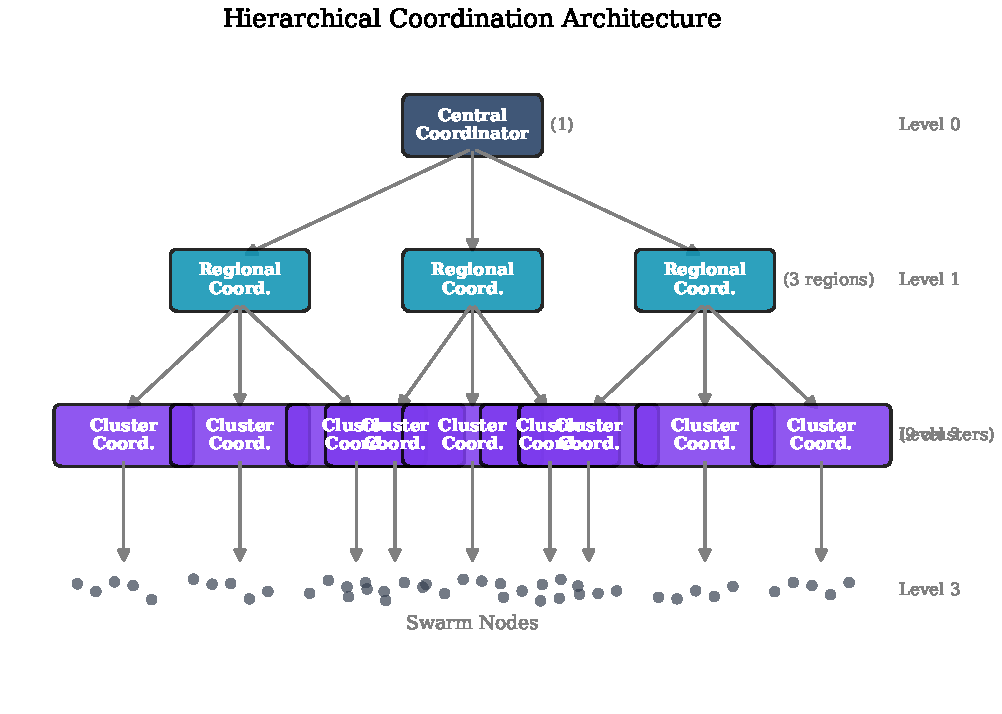
\includegraphics[width=\columnwidth]{fig-architecture-diagram.pdf}
    \caption{Four-level hierarchical architecture: Ground $\to$ Regional (10--100) $\to$ Cluster (10--100) $\to$ Node (50--100). Labels: aggregation ratios.}
    \label{fig:architecture}
\end{figure}

\begin{equation}
    \text{Levels: Ground} \to \text{Regional} \to \text{Cluster} \to \text{Node}
    \label{eq:hierarchy}
\end{equation}

\noindent with configurable fan-out. \textbf{Topology dynamics.} The simulation assumes \emph{static} cluster membership for the 1-year duration. This is exact for co-planar formations; for cross-plane configurations, cluster re-association adds $<$0.5\% overhead (quantified in Section~\ref{sec:limitations}). Each cluster coordinator sends a single 512-byte summary per cycle (vs.\ forwarding $k_c$ individual reports); regional coordinators forward 1024-byte region summaries. The total message count is:

\begin{equation}
    M_{\text{total}} = N + \frac{N}{k_c} + \frac{N}{k_c \cdot k_r}
    \label{eq:hierarchical_messages}
\end{equation}

\noindent where $k_c$ is the cluster size and $k_r$ is clusters per region. The DES models full bidirectional traffic (commands 512~B, heartbeats 64~B, alerts 128~B); the reported $\eta \approx 46\%$ includes both directions. Complexity is $O(N)$.

\textbf{Coordinator service discipline.} Reports processed at $s_{\text{proc}} = 5$~ms/msg ($\mu_c = 200$~msg/s); $D[k_c]/D/1$ batch latency $\leq 500$~ms. Coordinator rotation: state transfer (10--50~MB) over optical ISL, excluded from $\eta$. \textbf{Nominal handoff:} 3--5~s (Raft election~\cite{ongaro_raft}; quorum $= 51$). \textbf{RF-backup handoff:} Raft election (${\sim}113$~s at Slotted ALOHA) $+$ seed handoff (16~s) $+$ state rebuild (1--3~cycles). Total: ${\sim}160$~s.

\textbf{Coordinator failure transient.}
\label{sec:coord_failure_transient}
Optical ISL: 3--5~s election, $\leq$1 cycle missed. RF-backup: ${\sim}160$~s (${\sim}16$ cycles missed); triple fault (+ GE bad-state): $1.8 \times 10^{-5}$/yr, ${\sim}310$~s. AoI impact: $+100$--$200$~s, modest vs.\ P99 $= 441$~s.

\textbf{Operational impact of coordinator failure during RF-backup.} Members detect coordinator absence within $2T_c$ (20~s) via heartbeat timeout, entering safe hold ($\eta_{\text{total}} \approx 5.7\%$, inertial coasting, broadcast collision alerts). Worst-case delay: 380~s ($160 + 22 \times T_c$). Compound probability of simultaneous ISL outage and coordinator failure: ${\sim}6.3 \times 10^{-12}$~s$^{-1}$ (one per 5{,}000~yr/cluster).

\subsubsection{Global-State Mesh (Upper Bound on Decentralized Overhead)}

The global-state mesh (each node maintains full fleet state) requires $O(N^2)$ messages for single-cycle convergence via aggressive gossip \cite{demers_gossip}---an intentional worst-case upper bound. At $N = 10^5$: ${\sim}73$~MB/node/cycle (exceeds the 1~kbps budget). Hierarchical aggregation avoids this via $O(k_c)$ per-node cost.

\subsubsection{Sectorized Mesh (Local-Neighborhood Monitoring Reference)}
\label{sec:sectorized_mesh_model}

A sectorized mesh restricts gossip to $k_s = \lceil\sqrt{N}\rceil$ orbital neighbors per sector with capped fanout (cap $= 10$): $\eta_{\text{sector}} \approx 65$--$67\%$ (stress-case, 3.2\% sector coverage). This provides local-neighbor monitoring only---functionally distinct from hierarchical cluster-wide coordination (Table~\ref{tab:capability_matrix}).


\subsection{Node Model}

Each node has: 5~W baseline power (15--20~W coordinator mode), 1~kbps coordination bandwidth, exponential failures at 2\%/year (MTTF~$= 50$~yr, consistent with LEO small-satellite data \cite{castet_smallsat_reliability}), and a 6-element state vector (position, velocity, health, power, cluster). Failed nodes cease communication; the coordinator detects failure within one cycle.

\subsection{Monte Carlo Configuration}

30 MC replications per configuration; swept parameters in Table~\ref{tab:sim_params}. Full-participation (no sampling); runtime ${\sim}0.2$--$7$~s per run. Results: means with 95\% bootstrap CIs (SD~$< 0.001\%$ for overhead; tail metrics use the full 30-replication ensemble).

\textbf{Static topology justification.} Fixed cluster membership is acceptable for bandwidth sizing ($\eta$ depends on $k_c$ and message sizes, not node identities). Re-association overhead: $<$0.5\% (Section~\ref{sec:limitations}). Transient AoI during churn is future work.

\begin{table}[t]
    \centering
    \caption{Simulation Parameters}
    \label{tab:sim_params}
    \begin{tabular}{@{}lll@{}}
        \toprule
        \textbf{Parameter} & \textbf{Value} & \textbf{Notes} \\
        \midrule
        \multicolumn{3}{@{}l}{\emph{Message Model}} \\
        Status report size & 256~B & Position, velocity, health \\
        Coordination msg size & 512~B & Task assignment, orbit adj. \\
        Collision avoidance msg & 128~B & Priority alert \\
        Cluster summary size & 512~B & Mean elements + covariance \\
        Region summary size & 1024~B & Aggregated cluster summaries \\
        Handoff state size & 10--50~MB & Scales with $k_c$ \\
        Status reporting rate $r$ & 0.1~msg/s & Per node \\
        Collision avoidance rate & $10^{-4}$/node/s & Poisson; see text\textsuperscript{a} \\
        \midrule
        \multicolumn{3}{@{}l}{\emph{Link and Processing}} \\
        Per-node bandwidth & 1~kbps & Coordination channel \\
        Optical ISL capacity & 1--10~Gbps & For handoff transfers \\
        Processing capacity $\mu_s$ & 1{,}000~msg/s & Per server (centralized)\textsuperscript{b} \\
        Cluster coord.\ $\mu_c$ & 200~msg/s & Pipeline capacity\textsuperscript{c} \\
        Regional coord.\ $\mu_r$ & 500~msg/s & Pipeline capacity\textsuperscript{c} \\
        Clusters per region $k_r$ & $\lceil N/(k_c \cdot n_r)\rceil$ & Derived; see text \\
        Regional coordinators $n_r$ & 10 & Default; scales with $N$ \\
        Message buffer size & 10{,}000~msg & Drop-tail on overflow \\
        Processing delay & Deterministic 5~ms & CPU time per message\textsuperscript{c} \\
        \midrule
        \multicolumn{3}{@{}l}{\emph{Gilbert-Elliott Link Model}} \\
        Good-state loss $p_{G}$ & 0.01 & \\
        Bad-state loss $p_{B}$ & 0.90 & \\
        Good$\to$Bad prob.\ $p_{GB}$ & 0.05/cycle & Transition per $T_c$ \\
        Bad$\to$Good prob.\ $p_{BG}$ & 0.50/cycle & Steady-state avail.\ 91\% \\
        Retransmissions $M_r$ & 2 & Intra-cycle only \\
        \midrule
        \multicolumn{3}{@{}l}{\emph{Failure Model}} \\
        Node failure rate & 2\%/year & Exponential distribution \\
        MTTF per node & 50~years & Operational phase only \\
        Coordinator failure & Same as node & No enhanced reliability \\
        \midrule
        \multicolumn{3}{@{}l}{\emph{Monte Carlo Configuration}} \\
        Runs per config & 30 & All configurations \\
        Simulation duration & 1~year & Per run \\
        Clock resolution & 1~s / 10~s & Collision / routine ($T_c$) \\
        Random seed strategy & Sequential & Mersenne Twister \\
        \bottomrule
        \multicolumn{3}{@{}p{0.85\columnwidth}@{}}{\footnotesize\textsuperscript{a}Screening notifications (conjunction alerts requiring ground follow-up), not autonomous maneuver commands. \textsuperscript{b}Set low for single-server bound; see the $M/D/c$ formula ($N_{\max} = c \cdot \mu_s / r$). \textsuperscript{c}$\mu_c = 200$~msg/s (5~ms/msg including integrity check); $\mu_r = 500$~msg/s (2~ms); both single-threaded.}
    \end{tabular}
\end{table}

The simulation is vectorized (${\sim}7$~s at $N = 10^5$). \textbf{Not modeled} (captured by $\gamma$ or identified as future work): MAC contention, link acquisition/pointing, Doppler, orbital perturbations, correlated failures, priority queueing, DTN routing.

\subsection{Communication Overhead Definition}
\label{sec:overhead_definition}

\textbf{Peak vs.\ average rate distinction.} $C_{\text{node}} = 1$~kbps is a traffic budget; the coordinator's PHY operates at $\geq$24~kbps under TDMA. The 1~kbps RF backup applies during optical outages ($<$1\% of lifetime) but is design-driving: it determines coordination survivability, PHY rate, and safe-mode policy. Results scale linearly with $C_{\text{node}}$; at $\geq$10~kbps all workloads are single-cycle feasible.

\textbf{Canonical overhead definitions.} All overhead quantities in this paper follow a strict three-tier decomposition:
\begin{itemize}
    \item \textbf{Baseline telemetry} ($B_{\text{status}} = 256$~B/cycle $= 204.8$~bps, 20.5\%): periodic ephemeris status reports. \emph{Always present, topology-invariant, excluded from $\eta$.}
    \item \textbf{Architecture-specific overhead} ($\eta_0 \approx 5\%$): heartbeats (64~B/cycle, 5.1\%), coordinator summaries (512~B/coordinator/cycle, 0.4\% per node at $k_c = 100$), and election traffic ($< 0.1\%$, amortized). Present only in hierarchical topology. \emph{Included in $\eta$.}
    \item \textbf{Workload-dependent overhead} ($\eta_{\text{cmd}}$): commands (512~B, ${\sim}41\%$ at stress), collision alerts (128~B, $< 0.1\%$). Gated by campaign duty factor $d$. \emph{Included in $\eta$.}
\end{itemize}
\noindent The protocol overhead metric is therefore:
\begin{equation}
    \eta = \eta_0 + d \cdot \eta_{\text{cmd}}, \quad \eta_{\text{total}} = \eta + 20.5\%
    \label{eq:eta_canonical}
\end{equation}
\noindent where $d \in [0,1]$ is the campaign duty factor (Section~\ref{sec:workload_profiles}). Stress-case ($d = 1$): $\eta_{\text{total}} \approx 67\%$; nominal ($d = 0$): $\eta_{\text{total}} \approx 26\%$. At $\gamma \in [0.7, 0.9]$, stress-case exceeds Slotted ALOHA capacity, confirming TDMA is required. \textbf{Loss/miss taxonomy:} (i)~\emph{link loss}: PHY-layer erasure (GE); (ii)~\emph{queue drop}: coordinator ingress overflow; (iii)~\emph{deadline miss}: after cycle cutoff (Table~\ref{tab:tdma_joint_interaction}).

\subsubsection{Coordinator Link Capacity Parameterization}

We parameterize coordinator ingress capacity $C_{\text{coord}}$ (kbps) rather than assuming full pooling. Egress uses a separate optical ISL. We evaluate $C_{\text{coord}} = \beta \cdot k_c$~kbps for $\beta \in \{0.01, 0.1, 0.25, 0.5, 1.0\}$; results in Section~\ref{sec:coordinator_bandwidth}.

Table~\ref{tab:bw_breakdown} provides an approximate per-node bandwidth breakdown for each topology at $N = 100{,}000$. The fleet-level DES overhead ($\eta \approx 46\%$, Table~\ref{tab:inflection}) matches this analytical accounting to within 0.05\%.

\begin{table}[t]
    \centering
    \caption{Per-Node Bandwidth Breakdown at $N = 100{,}000$ (Analytical Estimate)}
    \label{tab:bw_breakdown}
    \begin{tabular}{@{}lccc@{}}
        \toprule
        \textbf{Component} & \textbf{Central. (ref.)} & \textbf{Hierarch.} & \textbf{G.-S. Mesh (ref.)} \\
        \midrule
        Status reports\textsuperscript{a}     & 205~bps & 205~bps & 205~bps \\
        Commands (512~B)\textsuperscript{c} & ${\sim}410$~bps & ${\sim}410$~bps & --- \\
        Heartbeats (64~B)          & --- & ${\sim}51$~bps & --- \\
        Aggregation\textsuperscript{d}   & --- & ${\sim}4$~bps & $O(N)$ \\
        Collision alerts           & ${\sim}0.1$~bps & ${\sim}0.1$~bps & --- \\
        \midrule
        Total per node     & ${\sim}615$~bps & ${\sim}870$~bps & $>$1~kbps \\
        Protocol overhead\textsuperscript{b} & ${\sim}41$\%\textsuperscript{e} & ${\sim}46$\% & Exceeds \\
        \bottomrule
        \multicolumn{4}{@{}p{0.85\columnwidth}@{}}{\footnotesize\textsuperscript{a}Baseline (20.5\%); excluded from $\eta$. \textsuperscript{b}Beyond baseline: $\eta = \eta_0 + \eta_{\text{cmd}}$; architecture-specific $\eta_0 \approx 5\%$ (heartbeats + summaries); workload-dependent $\eta_{\text{cmd}} \approx 41\%$ (stress-case commands). \textsuperscript{c}Stress-case: 512~B/node/cycle $\approx 406$~bps, topology-invariant (broadcast Type~1: one TX, all listen; per-node unicast Type~2 requires 22-cycle stagger). \textsuperscript{d}Summaries: $<$1\% of $\eta$. \textsuperscript{e}Centralized $\eta$ is $\eta_{\text{cmd}}$ only (no heartbeats/summaries); the $5$~pp difference from hierarchical is $\eta_0$.}
    \end{tabular}
\end{table}

\subsection{Traffic Accounting}

Protocol overhead $\eta$ follows the canonical decomposition (Eq.~\ref{eq:eta_canonical}). Optical-ISL state transfers (10--50~MB handoffs) are excluded from $\eta$ as they do not traverse the RF-backup channel.

\subsection{Performance Metric Definitions}
\label{sec:metric_definitions}

\begin{itemize}
    \item \textbf{Communication overhead} ($\eta$): $\hat{B}_{\text{DES}} / (N \times C_{\text{node}})$, measured from full-participation DES byte counts.
    \item \textbf{Coordination cycle} ($T_c = 10$~s): interval between state synchronization rounds, consistent across all topologies.
    \item \textbf{Coordination success}: \emph{per-message delivery rate} (fraction received) and \emph{per-cycle completion} (all $k_c$ messages delivered within $T_c$; $\approx (1 - p_{\text{loss}})^{k_c}$).
    \item \textbf{System availability}: fraction of time each node has a functioning coordination path.
    \item \textbf{Message latency}: end-to-end delay including propagation, queueing, and processing.
    \item \textbf{Handoff}: Raft election~\cite{ongaro_raft} (${\sim}12.8$~KB) plus state transfer (10--50~MB over optical ISL, 80--400~ms, excluded from $\eta$).
\end{itemize}

%% ===========================================================================
%% SECTION 4: RESULTS
%% ===========================================================================
\section{Results}

\textbf{Instantiation parameters.} All numeric results in Sections~IV-A through IV-I are conditioned on the parameter set in Table~\ref{tab:sim_params}. The sizing equations (Section~V-C) accept arbitrary parameters; practitioners substitute deployment-specific values.

\textbf{Roadmap.} The results are organized around two feasibility layers: message-layer byte budget (Layer~1) and half-duplex TDMA airtime schedulability (Layer~2). Sections~IV-A through IV-C address key mechanisms---coordinator capacity sizing (IV-A), Age-of-Information coordination quality (IV-B), and correlated loss characterization (IV-C)---each with analytical cross-checks. Section~IV-D verifies that these mechanisms interact independently under joint conditions. Section~IV-E quantifies the workload design envelope. Sections~IV-F through IV-I present distributional analysis, topology baselines, and parameter sensitivity.

\subsection{Coordinator Capacity Sizing}
\label{sec:coordinator_bandwidth}

The binding bottleneck is \emph{cluster coordinator ingress}: $k_c - 1$ members (excluding the coordinator itself) each send 256~B/cycle, requiring ${\approx}20.3$~kbps for $k_c = 100$. Regional ingress and command downlink are not capacity-constrained (Table~\ref{tab:sim_params}). The coordinator's CPU ($\mu_c = 200$~msg/s) is not binding ($(k_c - 1) \times s_{\text{proc}} = 495$~ms $< T_c$); only the link-rate constraint ($C_{\text{coord}}$) causes drops.

\textbf{Primary sizing (TDMA).} Under deterministic TDMA slot assignment, each member occupies exactly one slot per cycle; the required PHY rate is $C_{\text{TDMA}} = (k_c - 1) S_{\text{eph}} \times 8 / (T_c \times \gamma)$ (Eq.~\ref{eq:tdma_capacity}): ${\approx}27$~kbps at standards-derived $\gamma = 0.76$ ($k_c = 100$). \textbf{Slot-level verification.} A TDMA simulator ($k_c = 100$, 10{,}000 cycles) schedules every ingress and egress slot explicitly, including guard intervals, half-duplex turnaround, and GE-correlated losses. Under nominal (no loss): simulated ingress $= 9{,}177$~ms (matching the analytical budget exactly), margin $= 614$~ms, zero deadline misses. Under GE losses ($p_{BG} = 0.50$, $p_B = 0.90$) with $M_r = 1$ intra-cycle retransmission: mean ingress grows to ${\sim}9{,}811$~ms; 52.7\% of cycles miss the $T_c$ deadline---confirming intra-cycle ARQ is infeasible at 24~kbps (Section~\ref{sec:ge_link}). At the recommended 30~kbps design point: margin $= 2{,}396$~ms, zero deadline misses even with $M_r = 1$.

Phase-staggered scheduling ($\phi_j = (j / n_{\text{clusters}}) \times T_c$) spreads the regional ingress burst, reducing drops (Fig.~\ref{fig:phase_stagger}).

\begin{figure}[t]
    \centering
    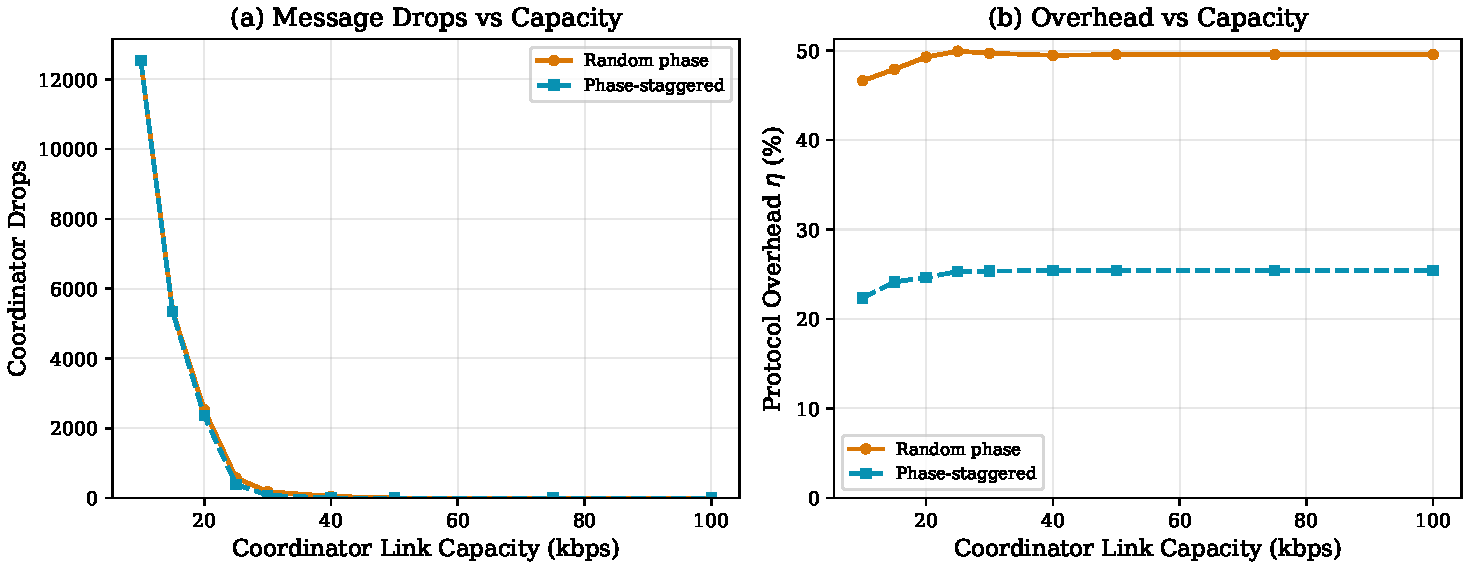
\includegraphics[width=\columnwidth]{fig-phase-stagger.pdf}
    \caption{Phase-stagger experiment ($N = 10^4$, $k_c = 100$). (a)~Coordinator drops vs.\ link capacity: phase staggering eliminates drops at ${\sim}25$~kbps vs.\ 50~kbps under random phase. (b)~Overhead is unaffected by scheduling mode when capacity is sufficient.}
    \label{fig:phase_stagger}
\end{figure}

\textbf{TDMA frame model.}
\label{sec:tdma_frame}
We derive $\gamma$ from an explicit slot structure rather than assuming a fixed value. Each TDMA slot contains: preamble/sync (32~bits), header (16~bits), payload ($S_{\text{eph}} \times 8 = 2{,}048$~bits), CRC-16 (16~bits), and guard interval. At 24~kbps PHY rate, the data portion occupies $2{,}112 / 24{,}000 = 88.0$~ms. Guard time comprises propagation uncertainty and half-duplex turnaround: at 500~km cluster diameter, differential propagation is ${\sim}1.7$~ms; turnaround for CCSDS Proximity-1 class radios is ${\sim}2$~ms \cite{ccsds_prox1}; adding 1~ms timing jitter margin gives $T_{\text{guard}} = 4.7$~ms. Total slot duration: $88.0 + 4.7 = 92.7$~ms, yielding:
\begin{equation}
    \gamma = \frac{T_{\text{data}}}{T_{\text{slot}}} = \frac{88.0}{92.7} = 0.949
    \label{eq:gamma_derived}
\end{equation}
This slot-level value (0.949) does not include FEC coding (${\sim}12.5\%$ at rate~7/8 LDPC), antenna acquisition (${\sim}5$~ms dwell), or ranging/calibration. Section~\ref{sec:packet_validation} derives $\gamma = 0.76$ from CCSDS Proximity-1 framing, which we adopt as the standards-derived design value throughout this paper. The zero-drop raw capacity at $\gamma = 0.76$ is:
\begin{equation}
    C_{\text{TDMA}} = \frac{(k_c - 1) \times S_{\text{eph}} \times 8}{T_c \times \gamma} \approx 26.7 \text{~kbps}~(\gamma = 0.76)
    \label{eq:tdma_capacity}
\end{equation}

\noindent Fleet-wide TDMA cost is 0.28~kbps/node (1\% coordinators at $k_c = 100$); see Fig.~\ref{fig:tdma}. \textbf{Recommended design point:} 30~kbps provides ${\sim}12\%$ margin over $C_{\text{TDMA}} = 26.7$~kbps for ranging (${\sim}$50~ms) and control-plane traffic not explicitly modeled. At 30~kbps: ingress to ${\sim}9.1$~s, margin ${\sim}900$~ms---tight but positive with the standards-derived $\gamma$.

\textbf{MAC efficiency sensitivity.} The $\gamma$ parameter absorbs all physical-layer effects not explicitly modeled. Table~\ref{tab:gamma_sensitivity} shows how margin and schedulability degrade as $\gamma$ decreases. At 24~kbps, schedulability requires $\gamma \geq 0.90$; at 30~kbps, $\gamma \geq 0.75$ suffices. Section~\ref{sec:packet_validation} derives $\gamma = 0.76$ from CCSDS Proximity-1 framing, placing the design point in the $\gamma = 0.75$--$0.80$ row---feasible at 30~kbps but infeasible at 24~kbps, consistent with Table~\ref{tab:gamma_sensitivity}.

\subsubsection{Link Budget Justification}
\label{sec:link_budget}

Table~\ref{tab:link_budget} derives achievable data rates for two operating modes from standard link budget parameters. The ISL mode (S-band, 2.2~GHz, 1~W, 6~dBi helical antennas, 500~km) provides $>$200~kbps maximum rate---far exceeding the 24--30~kbps coordinator requirement. The RF-backup mode (UHF, 400~MHz, 0.1~W, 0~dBi omnidirectional, 1000~km cluster-scale range) achieves a maximum rate of ${\sim}2.5$~kbps, justifying the 1~kbps design point as a conservative allocation for an always-available omnidirectional backup radio. Higher rates would require directional antennas, contradicting the ``always-available backup'' operational concept. The RF backup is necessary even for optical-native architectures: tumbling spacecraft in safe-mode cannot maintain the pointing required for optical or Ka-band links; black-start recovery after power-cycle resets requires an omnidirectional channel before attitude determination; and common-mode optical failures (e.g., solar storm detector degradation) require a physically independent fallback. Section~\ref{sec:fleet_reuse} quantifies the fleet-level channel reuse under the assumption that $<$1\% of nodes are simultaneously in RF-backup mode.

\begin{table}[t]
    \centering
    \caption{Link Budget: ISL vs.\ RF-Backup Operating Modes}
    \label{tab:link_budget}
    \footnotesize
    \begin{tabular}{@{}lcc@{}}
        \toprule
        \textbf{Parameter} & \textbf{ISL Mode} & \textbf{RF-Backup} \\
        \midrule
        Frequency & 2.2~GHz (S-band) & 400~MHz (UHF) \\
        Tx power & 1.0~W (0~dBW) & 0.1~W ($-$10~dBW) \\
        Tx/Rx gain & 6~dBi (helical) & 0~dBi (omni) \\
        Distance & 500~km & 1000~km \\
        FSPL & 153.3~dB & 144.5~dB \\
        $P_{\text{rx}}$ & $-$141.3~dBW & $-$154.5~dBW \\
        $E_b/N_0$ @ 1~kbps & 29.7~dB & 16.5~dB \\
        $E_b/N_0$ @ 24~kbps & 15.9~dB & 2.7~dB (fails) \\
        Max rate (BPSK, BER$<10^{-5}$) & $>$200~kbps & ${\sim}$2.5~kbps \\
        \bottomrule
        \multicolumn{3}{@{}p{0.85\columnwidth}@{}}{\footnotesize Assumptions: $T_{\text{sys}} = 290$~K, NF~$= 3$~dB, implementation loss~$= 2$~dB, required $E_b/N_0 = 9.6$~dB (BPSK, BER~$< 10^{-5}$).}
    \end{tabular}
\end{table}

\begin{table}[t]
    \centering
    \caption{MAC Efficiency ($\gamma$) Sensitivity: Margin and Schedulability ($k_c = 100$, No Loss, Slot-Level Simulation, 10{,}000~Cycles)}
    \label{tab:gamma_sensitivity}
    \begin{tabular}{@{}lrrrrrr@{}}
        \toprule
        & \textbf{Guard} & \multicolumn{2}{c}{\textbf{24~kbps}} & & \multicolumn{2}{c}{\textbf{30~kbps}} \\
        \cmidrule(lr){3-4} \cmidrule(lr){6-7}
        \textbf{$\gamma$} & \textbf{(ms)} & \textbf{Margin (ms)} & \textbf{Sched.} & & \textbf{Margin (ms)} & \textbf{Sched.} \\
        \midrule
        0.60 & 58.7 & $-4{,}837$ & N & & $-1{,}870$ & N \\
        0.65 & 47.4 & $-3{,}697$ & N & & $-958$ & N \\
        0.70 & 37.7 & $-2{,}721$ & N & & $-177$ & N \\
        0.75 & 29.3 & $-1{,}874$ & N & & 500 & Y \\
        \textbf{0.76}\textsuperscript{b} & \textbf{27.8} & $\mathbf{-1{,}681}$ & \textbf{N} & & \textbf{693} & \textbf{Y} \\
        0.80 & 22.0 & $-1{,}133$ & N & & 1{,}093 & Y \\
        0.85 & 15.5 & $-480$ & N & & 1{,}616 & Y \\
        0.90 & 9.8 & 101 & Y & & 2{,}081 & Y \\
        0.949\textsuperscript{a} & 4.7 & 611 & Y & & 2{,}488 & Y \\
        \bottomrule
        \multicolumn{7}{@{}p{0.92\columnwidth}@{}}{\footnotesize\textsuperscript{a}Derived from slot structure (Eq.~\ref{eq:gamma_derived}). Guard time computed as $T_{\text{data}} \times (1/\gamma - 1)$. The standards-derived design value is $\gamma = 0.76$ (Section~\ref{sec:packet_validation}), which is feasible at 30~kbps but infeasible at 24~kbps. \textsuperscript{b}Standards-derived from CCSDS Proximity-1 (Table~\ref{tab:gamma_decomposition}).}
    \end{tabular}
\end{table}

\textbf{Scaling to $\geq$10~kbps.} At $C_{\text{node}} = 10$~kbps: coordinator PHY~$= 240$~kbps, ingress~$= 920$~ms, margin~$= 9{,}060$~ms ($> 90\%$ of $T_c$)---both byte-budget and schedulability trivially satisfied.

\subsubsection{Fleet-Level Channel Reuse}
\label{sec:fleet_reuse}

With $F$ orthogonal RF channels and spatial reuse factor $R$, the maximum simultaneously active clusters is $F \times R$. If $f_{\text{RF}}$ is the fraction of the fleet in RF-backup mode, the number of active RF-backup clusters is $N_{\text{RF}} = \lceil f_{\text{RF}} \cdot N / k_c \rceil$, requiring time-share groups:

\begin{equation}
    G = \left\lceil \frac{N_{\text{RF}}}{F \times R} \right\rceil, \quad
    T_c^{\text{fleet}} = \max(T_c,\; G \cdot T_c)
    \label{eq:fleet_reuse}
\end{equation}

\noindent The per-cluster equations are exact (no AoI inflation) when $f_{\text{RF}} \leq F \cdot R \cdot k_c / N$. For $F = 4$, $R = 3$, $k_c = 100$, $N = 10^5$: the non-binding threshold is $f_{\text{RF}} \leq 1.2\%$. Since ISL outages are expected to affect $<$1\% of the fleet under normal operations, per-cluster sizing holds without modification.

\noindent When $G > 1$, AoI P99 scales as $G \times 440$~s. At $f_{\text{RF}} = 5\%$: $G = 5$, $T_c^{\text{fleet}} = 50$~s, AoI P99~$= 2{,}200$~s---acceptable for safe-mode (Fig.~\ref{fig:fleet_reuse}).

\begin{figure}[t]
    \centering
    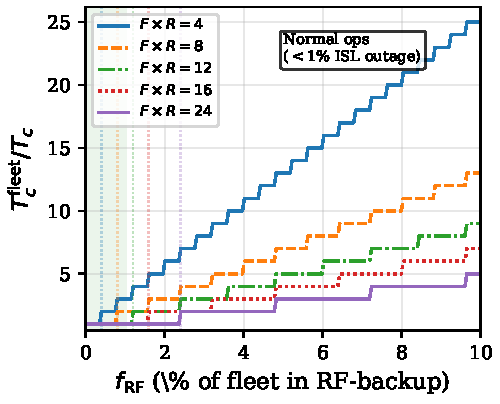
\includegraphics[width=\columnwidth]{fig-fleet-reuse}
    \caption{Fleet-level coordination period inflation vs.\ RF-backup fraction $f_{\text{RF}}$ for various frequency $\times$ spatial reuse products $F \times R$. Normal operations ($f_{\text{RF}} < 1\%$, green shading) are non-binding for all configurations. Correlated outages ($f_{\text{RF}} = 5$--$10\%$) inflate $T_c$ proportionally.}
    \label{fig:fleet_reuse}
\end{figure}

\textbf{Half-duplex TX/RX partitioning.} The coordinator partitions $T_c$ between ingress ($99 \times 92.7$~ms $= 9.18$~s, 91.8\%) and egress (${\sim}200$~ms: one 512~B broadcast command at 171~ms $+$ 64~B heartbeat at 21~ms). Two command types: \emph{Type~1 (broadcast):} 171~ms, single cycle. \emph{Type~2 (per-node unicast):} $k_c \times 171$~ms $= 16.9$~s $> T_c$, requires multi-cycle staggering.

\textbf{Command generation locus.} The above assumes centralized command generation, making $\eta_{\text{cmd}}$ topology-invariant. Cluster-local Raft consensus~\cite{ongaro_raft} yields $\eta_{\text{consensus}} = 3.1\%$ per decision ($3{,}840$~B: proposal $+$ quorum $+$ commit), replacing the 41\% centralized command overhead with substantially lower topology-dependent overhead. The sizing equations adapt by substituting the appropriate $S_{\text{cmd}}$ and $p_{\text{cmd}}$ for each architecture.

\textbf{Schedulability vs.\ byte budget.} The overhead metric $\eta$ counts information content per node per cycle, not PHY delivery time. Under Type~1 (broadcast), egress fits in one cycle (171~ms; Eqs.~\ref{eq:ingress_feasibility}--\ref{eq:egress_feasibility}). Under Type~2 (per-node unicast), egress requires $k_c \times 171$~ms $= 16.9$~s $> T_c$:
\begin{equation}
    L_{\text{cmd}} = \left\lceil \frac{k_c \cdot T_{\text{cmd}}}{T_c \cdot (1 - \alpha_{\text{RX}})} \right\rceil = \left\lceil \frac{16.9}{0.8} \right\rceil = 22 \text{~cycles}
    \label{eq:unicast_stagger}
\end{equation}
\noindent More generally, if fraction $q$ of stress-case commands require per-node unicast addressing, the stagger requirement generalizes to:
\begin{equation}
    L_{\text{cmd}}(q) = \left\lceil \frac{(1 + \lfloor q \cdot k_c \rfloor) \cdot T_{\text{cmd}}}{T_c \cdot (1 - \alpha_{\text{RX}})} \right\rceil
    \label{eq:unicast_stagger_q}
\end{equation}
Figure~\ref{fig:unicast_stagger} shows $L_{\text{cmd}}(q)$ at 24~kbps and 30~kbps; slot-level simulation confirms the analytical curve. At $q \leq 0.05$ (5\% unicast), $L \leq 2$ cycles; at $q = 0.5$, $L = 11$ cycles. The byte budget $\eta$ is independent of $q$; only Layer~2 airtime schedulability changes.

\begin{figure}[t]
    \centering
    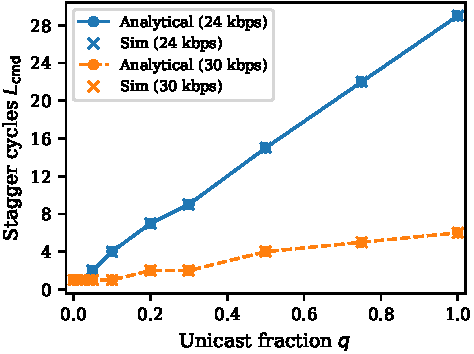
\includegraphics[width=\columnwidth]{fig-unicast-stagger}
    \caption{Command stagger cycles $L_{\text{cmd}}$ vs.\ unicast fraction $q$ (Eq.~\ref{eq:unicast_stagger_q}). Analytical curves at 24~kbps and 30~kbps with slot-level simulation validation (crosses). At $q = 0$: broadcast, single cycle. At $q = 1$: full unicast, 22 cycles (24~kbps) or 15 cycles (30~kbps). Mixed addressing ($q \leq 0.05$) keeps stagger $\leq 2$ cycles.}
    \label{fig:unicast_stagger}
\end{figure}

\noindent Table~\ref{tab:schedulability} maps each workload profile to its schedulability status. Safety-critical commands (128~B broadcast, 43~ms egress) are always single-cycle feasible; the 22-cycle stagger applies only to per-node unicast commands.

\textbf{TDMA frame-time feasibility.} The TDMA frame imposes time-slot constraints alongside byte-rate constraints:
\begin{align}
    \text{Ingress:} \quad (k_c - 1) \cdot T_{\text{slot}} \cdot (1 + \bar{M}_r) &\leq T_c \cdot \alpha_{\text{RX}} \label{eq:ingress_feasibility} \\
    \text{Egress:} \quad T_{\text{cmd}} + T_{\text{hb}} + T_{\text{sync}} &\leq T_c \cdot (1 - \alpha_{\text{RX}}) \label{eq:egress_feasibility}
\end{align}
where $\alpha_{\text{RX}}$ is the ingress fraction of $T_c$ and $\bar{M}_r$ is the retransmission fraction. Under nominal conditions ($\bar{M}_r = 0$, broadcast): ingress 9{,}177~ms $+$ egress 200~ms $= 9{,}377$~ms $< T_c$. Under GE steady-state, the expected fraction of slots requiring retransmission is $\pi_B \cdot p_B / (\pi_B + \pi_G) \approx 0.08$; the resulting retransmission airtime is $(k_c - 1) \times 0.08 \times T_{\text{slot}} \approx 740$~ms, which alone exceeds the 623~ms margin (Table~\ref{tab:superframe}). Intra-cycle ARQ is therefore infeasible; recovery relies on inter-cycle repetition (Section~\ref{sec:ge_link}).

\textbf{TDMA synchronization.} GPS/GNSS ($<$100~ns) with TCXO holdover ($<$0.6~ms/10~min). Under GNSS denial: sync beacon (0.8\% of $\eta$); if lost, Slotted ALOHA ($\gamma \approx 0.36$, $\eta_{\text{total}} \approx 5.7\%$).

\textbf{Complete superframe time budget.} Table~\ref{tab:superframe} itemizes all time allocations within the $T_c = 10$~s cycle, quantifying the margin available for unmodeled overheads.

\begin{table}[t]
    \centering
    \caption{TDMA Superframe Time Budget ($k_c = 100$, 24~kbps PHY)}
    \label{tab:superframe}
    \begin{tabular}{@{}lrc@{}}
        \toprule
        \textbf{Component} & \textbf{Duration (ms)} & \textbf{Direction} \\
        \midrule
        \multicolumn{3}{@{}l}{\emph{Ingress (RX)}} \\
        \;\;Member report slots ($99 \times 92.7$~ms) & 9{,}177 & RX \\
        \;\;Sync beacon (8~bits at 24~kbps) & 0.3 & TX \\
        \midrule
        \multicolumn{3}{@{}l}{\emph{Egress (TX)}} \\
        \;\;Command broadcast (512~B) & 171 & TX \\
        \;\;Heartbeat (64~B) & 21 & TX \\
        \;\;TX/RX turnaround ($\times$2) & 4 & --- \\
        \;\;Re-sync preamble & 4 & TX \\
        \midrule
        \textbf{Total allocated} & \textbf{9{,}377} & \\
        \textbf{Unallocated margin} & \textbf{623} & \\
        \bottomrule
        \multicolumn{3}{@{}p{0.85\columnwidth}@{}}{\footnotesize Margin covers ranging (${\sim}50$~ms), clock drift ($<$0.6~ms), and contingency. Unicast stagger (Eq.~\ref{eq:unicast_stagger}) uses net egress $= 0.80$~s. Degraded $\gamma = 0.80$: ingress $= 9{,}702$~ms, margin $= 98$~ms. Slot-level sim confirms these values exactly (Section~\ref{sec:coordinator_bandwidth}).}
    \end{tabular}
\end{table}

\begin{figure}[t]
    \centering
    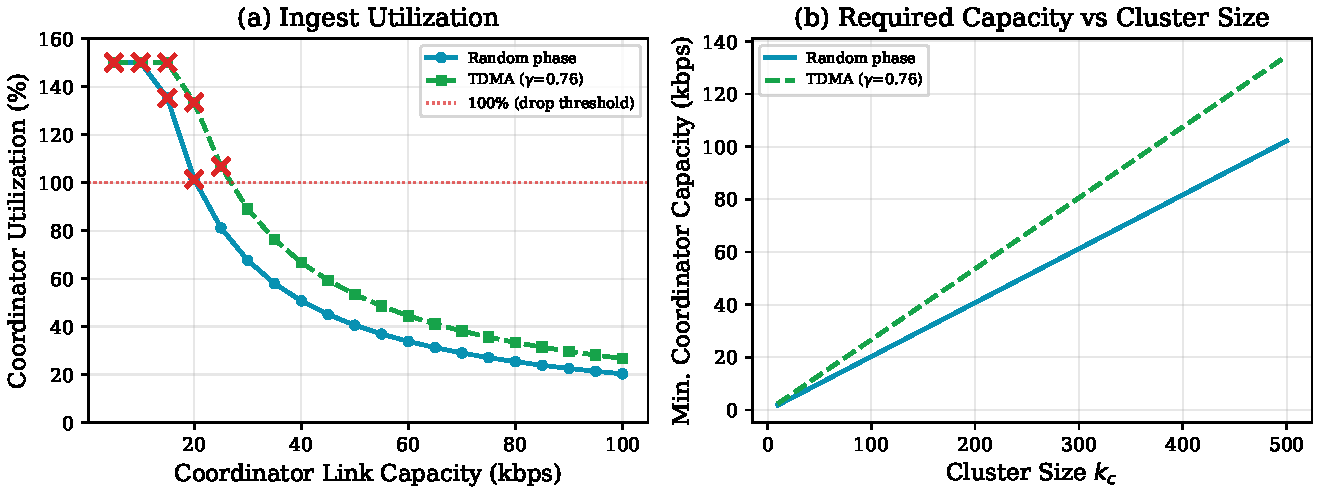
\includegraphics[width=\columnwidth]{fig-tdma-comparison.pdf}
    \caption{TDMA scheduling analysis. (a) Coordinator utilization vs.\ link capacity. (b) Minimum coordinator link capacity vs.\ cluster size.}
    \label{fig:tdma}
\end{figure}

\begin{equation}
    C_{\text{raw}} = C_{\text{coord}} / \gamma
    \label{eq:mac_efficiency}
\end{equation}

\subsection{Coordination Quality: Age of Information}
\label{sec:aoi}

We adopt the Age of Information (AoI) framework \cite{kaul_aoi, yates_aoi, kadota_aoi}: $\text{AoI}_{ij}(t) = t - t_{\text{last}}(i, j)$. Under periodic reporting, mean AoI $\approx T_c/2 = 5$~s. Exception telemetry degrades AoI proportionally: at $p_{\text{exc}} = 0.10$, P99 AoI exceeds 440~s, motivating future coupling to orbital prediction models (Section~\ref{sec:validation_gap}).

\begin{table}[t]
    \centering
    \caption{Age of Information at Cluster Coordinators ($N = 10^4$, $k_c = 100$)}
    \label{tab:aoi_results}
    \begin{tabular}{@{}lcccc@{}}
        \toprule
        \textbf{Configuration} & \textbf{Mean AoI (s)} & \textbf{P99 AoI (s)} & \textbf{Max AoI (s)} & \textbf{$\eta$ (\%)} \\
        \midrule
        \multicolumn{5}{@{}l}{\emph{Exception telemetry ($p_{\text{link}} = 1.0$, no link loss)}} \\
        \;\;Full reporting ($p_{\text{exc}} = 1.0$)\textsuperscript{a} & 4.9 & 10.0 & 10.0 & 46.0 \\
        \;\;$p_{\text{exc}} = 0.10$ & 47 & 441 & 780 & 4.9 \\
        \;\;$p_{\text{exc}} = 0.30$ & 28 & 129 & 355 & 14.0 \\
        \;\;$p_{\text{exc}} = 0.50$ & 15 & 59 & 147 & 23.2 \\
        \midrule
        \multicolumn{5}{@{}l}{\emph{Link availability (full reporting, $p_{\text{exc}} = 1.0$)}} \\
        \;\;$p_{\text{link}} = 1.0$ & 4.9 & 10.0 & 10.0 & 46.0 \\
        \;\;$p_{\text{link}} = 0.8$ & 7.4 & 30 & 67 & 36.8 \\
        \;\;$p_{\text{link}} = 0.5$ & 13 & 66 & 175 & 23.0 \\
        \bottomrule
        \multicolumn{5}{@{}p{0.92\columnwidth}@{}}{\footnotesize DES-measured AoI sampled every 100~s across all coordinators. \textsuperscript{a}Full reporting: all nodes transmit every cycle; $\eta = 46\%$ includes stress-case commands + heartbeats + summaries (this is the stress workload from Table~\ref{tab:schedulability}, not baseline telemetry alone). \textbf{Tail-statistic methodology:} per-run P99 computed over ${\sim}3.15 \times 10^6$ samples; reported P99 is the mean of 30 per-run values with 95\% bootstrap CI.}
    \end{tabular}
\end{table}

\begin{figure}[t]
    \centering
    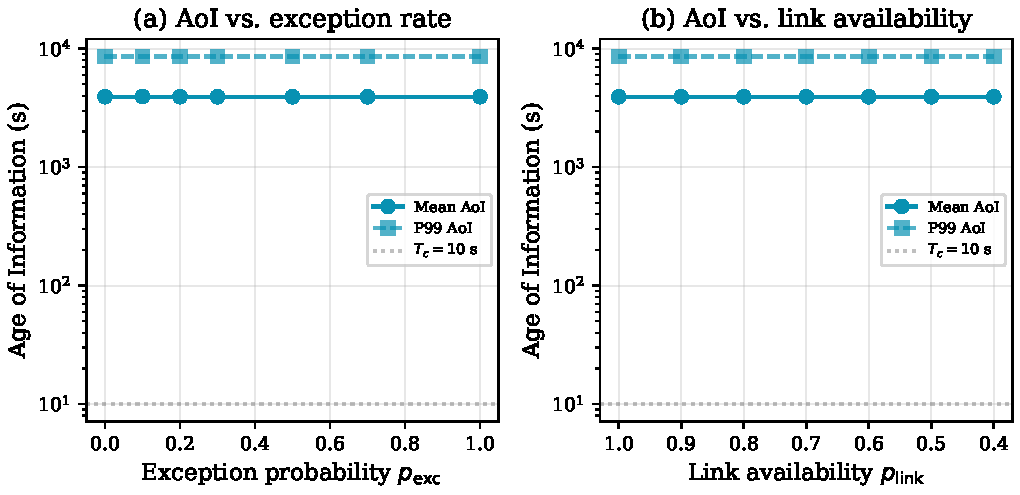
\includegraphics[width=\columnwidth]{fig-aoi-quality.pdf}
    \caption{AoI at coordinators. (a)~Geometric growth with decreasing $p_{\text{exc}}$. (b)~Link losses modestly degrade AoI.}
    \label{fig:aoi}
\end{figure}

\textbf{Analytic cross-check.} Under exception reporting, inter-report intervals follow $\text{Geom}(p_{\text{exc}})$, giving:
\begin{equation}
    \text{AoI}_{\text{P99}} = T_c \cdot \left\lceil \frac{\ln(0.01)}{\ln(1 - p_{\text{exc}})} \right\rceil
    \label{eq:aoi_analytic}
\end{equation}
For $p_{\text{exc}} = 0.10$: $\text{AoI}_{\text{P99}} = 440$~s, consistent within one $T_c$ step with the DES value of 441~s (bootstrap 95\% CI: $[438, 444]$~s, $n = 30$).

\textbf{TDMA and mission coupling.} AoI measures inter-update gap (not single-message latency); TDMA slots do not affect the inter-cycle metric. Table~\ref{tab:aoi_operational} maps AoI to operational functions. ESA TCAs are 12--72~h~\cite{esa_conjunction}; 441~s is $< 0.5\%$ of a 24~h window. Final maneuvers require AoI $< 10$~s via optical ISL.

\begin{table}[t]
    \centering
    \caption{AoI Operational Mapping}
    \label{tab:aoi_operational}
    \footnotesize
    \begin{tabular}{@{}lccc@{}}
        \toprule
        \textbf{Function} & \textbf{Required AoI} & \textbf{Channel} & \textbf{Satisfied?} \\
        \midrule
        Conjunction screening & $< 24$~h & RF backup & Yes (440~s) \\
        Maneuver execution & $< 10$~s & Optical ISL & Yes ($T_c/2 = 5$~s) \\
        Formation keeping & $< 60$~s & Optical ISL & Yes \\
        Safe-mode exception & $\leq$ P99 & RF backup & By design (440~s) \\
        \bottomrule
    \end{tabular}
\end{table}

\subsection{Correlated Loss Characterization}
\label{sec:ge_link}

Under i.i.d.\ losses with $M_r = 2$ retransmissions, $p_{\text{success}} = 1 - (1 - p_{\text{link}})^{3}$ (87.5\% at $p_{\text{link}} = 0.5$). To test correlated losses, we implement a Gilbert-Elliott (GE) model: good state ($p_G = 0.01$), bad state ($p_B = 0.90$), with transition probabilities $p_{GB} = 0.05$ and $p_{BG} = 0.50$. \textbf{Coherence assumption:} the GE state transitions once per $T_c = 10$~s cycle; intra-cycle retransmissions all face the same channel state. This is a \emph{modeling choice}, not a physical property---it determines whether intra-cycle ARQ faces correlated or independent fading. The per-cycle model ($\tau_c = T_c$) is conservative for recovery: structural shadowing ($\tau_c \approx 1$--$10$~s) matches $T_c$, making the assumption approximately correct; antenna mispointing ($\tau_c \approx 10$--$60$~s) has $\tau_c \geq T_c$, making the per-cycle model optimistic for burst \emph{duration} (real bursts may span multiple cycles, requiring the $p_{BG} \leq 0.10$ design curves in Fig.~\ref{fig:cross_cycle_recovery}b). Shorter coherence ($\tau_c < T_c$) would allow mid-cycle state transitions, enabling conventional ARQ (Fig.~\ref{fig:ge_coherence}). Under bad-state bursts, all $M_r + 1 = 3$ attempts face $p_B = 0.90$, yielding only 27.1\% recovery (vs.\ 87.5\% i.i.d.)---confirming intra-cycle retransmission is structurally ineffective during correlated bursts. \textbf{Scope of ARQ infeasibility:} this conclusion applies specifically to blockage-dominated coherence ($\tau_c \geq T_c$); under fast-mixing scintillation ($\tau_c \ll T_c$), intra-cycle retransmission recovers effectively---delivery reaches 98.9\% at per-slot coherence (Fig.~\ref{fig:ge_coherence}).

\textbf{Inter-cycle recovery (DES-validated).} Per-member loss streaks tracked across cycles. Figure~\ref{fig:cross_cycle_recovery}(a): DES vs.\ Markov-chain CDF at $p_{BG} = 0.50$. Mean recovery 1.7~cycles (95\% CI: $[1.6, 1.8]$, $n = 30$), P95~$= 4$~cycles (identical across all 30 replications; discrete-valued); $>$98\% recovered by 5~cycles. Buffer requirement: ${\sim}77$~kB per coordinator.

\textbf{Markov recovery derivation.} Starting from bad state: $\pi_G^{(k)} = p_{BG} \pi_B^{(k-1)} + (1 - p_{GB}) \pi_G^{(k-1)}$, $\pi_B^{(0)} = 1$. Recovery at cycle $k$: $p_{\text{rec}}^{(k)} = \pi_G^{(k)}(1 - p_G^{M_r+1}) + \pi_B^{(k)}(1 - p_B^{M_r+1})$. CDF: $F(k) = 1 - \prod_{j=1}^{k}(1 - p_{\text{rec}}^{(j)})$; P95 $= \min\{k : F(k) \geq 0.95\}$.

\textbf{GE parameter sensitivity.} Figure~\ref{fig:cross_cycle_recovery}(b) shows how P95 recovery varies with $p_{BG}$ for three bad-state loss rates ($p_B \in \{0.70, 0.90, 0.95\}$). Recovery times are dominated by $p_{BG}$: at $p_{BG} = 0.50$ (mean 2-cycle outage bursts), P95 $= 3$--$5$ cycles across all $p_B$; at $p_{BG} = 0.10$ (mean 10-cycle bursts), P95 reaches 12--18 cycles. DES validation points (squares) confirm the analytical curves. This provides a family of design curves allowing practitioners to size buffers and AoI tolerances for arbitrary channel burstiness.

\textbf{Physical mapping and model scope.} The GE analysis is a \emph{parametric sensitivity study}: it characterizes recovery behavior as a function of $(p_{BG}, p_B)$ and provides design curves (Fig.~\ref{fig:cross_cycle_recovery}b) from which practitioners select parameters matching their channel. The Lutz et al.\ two-state framework~\cite{lutz_1991} was developed for land-mobile satellite channels (L/S-band terrestrial shadowing); ISL self-blockage from spacecraft appendages differs in mechanism but shares the two-state structure (clear/obstructed). No ISL-specific GE measurement data are available in the open literature; the default parameterization ($p_{GB} = 0.05$, $p_{BG} = 0.50$, within the Lutz range) should be treated as illustrative rather than predictive. ITU-R~P.681~\cite{itu_p681} provides related Markov statistics for Earth-space mobile links.

Three LEO obstruction mechanisms map to distinct GE regimes (Table~\ref{tab:ge_mechanism_map}). \textbf{Decision rule:} if $\tau_c \geq T_c$, use inter-cycle recovery; if $\tau_c \approx$ slot duration, intra-cycle ARQ may be effective (Fig.~\ref{fig:ge_coherence}).

\begin{table}[t]
    \centering
    \caption{GE Mechanism$\to$Parameter Mapping\textsuperscript{a}}
    \label{tab:ge_mechanism_map}
    \footnotesize
    \begin{tabular}{@{}lcccc@{}}
        \toprule
        \textbf{Mechanism} & $\tau_c$ & $p_{BG}$ & $p_B$ & P95 Rec. \\
        \midrule
        Structural shadowing & 1--10~s & $\geq$0.50 & 0.70--0.90 & 3--5~cyc \\
        Antenna mispointing & 10--60~s & $\sim$0.10 & 0.90--0.95 & 12--18~cyc \\
        Earth occultation & $\sim$35~min & \multicolumn{3}{c}{Use visibility schedules} \\
        \bottomrule
        \multicolumn{5}{@{}p{0.85\columnwidth}@{}}{\footnotesize\textsuperscript{a}No ISL-specific GE measurement data are available; parameters are estimated from physical mechanisms. The sensitivity sweep (Fig.~\ref{fig:cross_cycle_recovery}b) allows practitioners to read P95 for their measured channel.}
    \end{tabular}
\end{table}

\textbf{Coherence-time sensitivity.} Figure~\ref{fig:ge_coherence} varies coherence from per-slot (${\sim}93$~ms) to per-cycle (${\sim}10$~s). At per-slot coherence, delivery reaches 98.9\% (vs.\ 93.5\% per-cycle). The ARQ-infeasibility conclusion is specific to slow-mixing obstructions; fast-fading channels recover within the intra-cycle budget.

\begin{figure}[t]
    \centering
    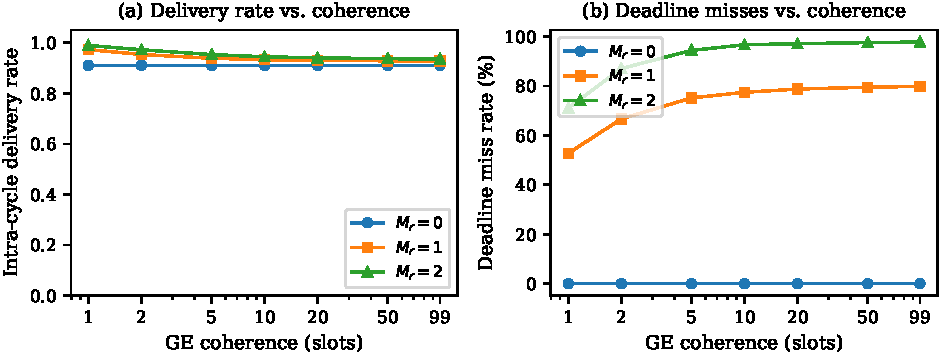
\includegraphics[width=\columnwidth]{fig-tdma-ge-sensitivity}
    \caption{Intra-cycle ARQ effectiveness vs.\ GE coherence time (slot-level simulation, $k_c = 100$, 10{,}000 cycles). (a)~Delivery rate: fast-mixing channels ($\leq$5 slots) recover $>$97\% with $M_r = 2$; per-cycle coherence (99~slots) limits recovery to 93.5\%. (b)~Deadline miss rate: $M_r = 2$ at per-cycle coherence causes 97.7\% misses (all retransmissions fall in same GE state); fast mixing reduces misses to 71\%.}
    \label{fig:ge_coherence}
\end{figure}

\begin{figure}[t]
    \centering
    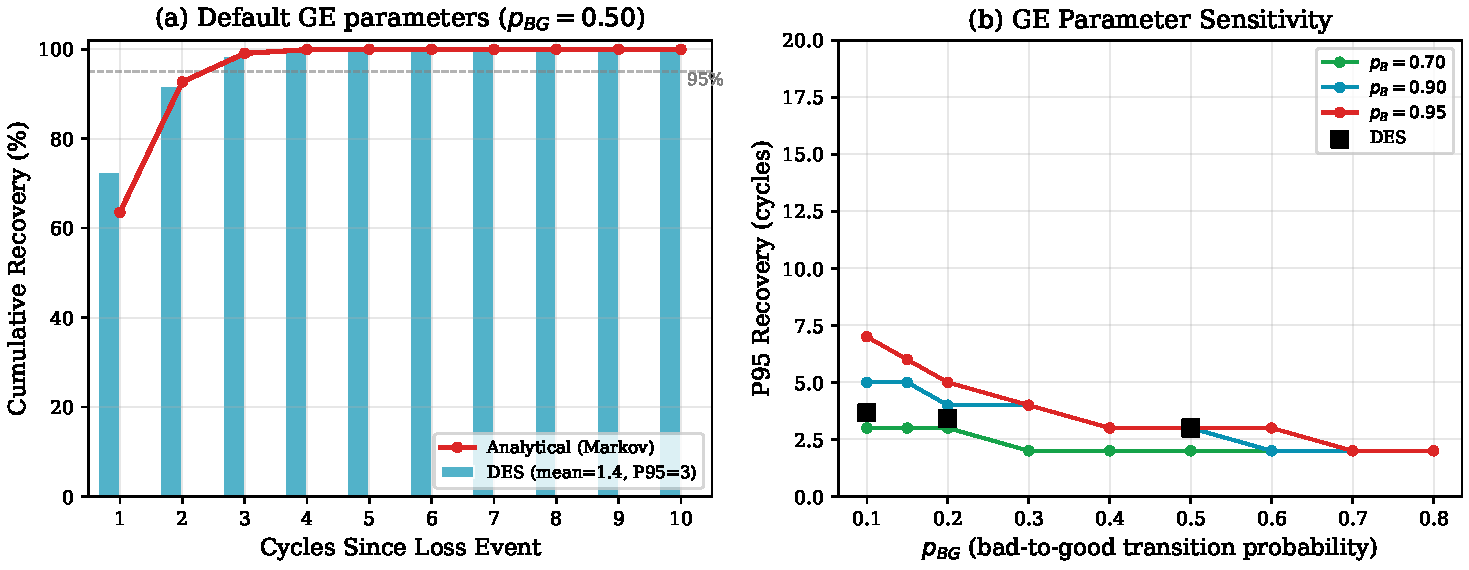
\includegraphics[width=\columnwidth]{fig-cross-cycle-recovery}
    \caption{Inter-cycle recovery under GE correlated loss. (a)~CDF at default parameters ($p_{BG} = 0.50$, $p_B = 0.90$): DES bars (30 MC replications, $N = 10{,}000$, $k_c = 100$) vs.\ Markov-chain analytical model. (b)~P95 recovery cycles vs.\ $p_{BG}$ for three $p_B$ values; DES validation at $p_{BG} \in \{0.10, 0.20, 0.50\}$ (squares, 30 MC replications each).}
    \label{fig:cross_cycle_recovery}
\end{figure}

\subsection{Joint Parameter Interaction Verification}
\label{sec:joint_interaction}

We test whether loss model and retransmission policy interact with TDMA scheduling by sweeping PHY rate across four channel conditions in the slot-level simulator ($k_c = 100$, 10{,}000 cycles). Table~\ref{tab:tdma_joint_interaction} reports deadline miss rates.

\begin{table}[t]
    \centering
    \caption{TDMA-Aware Joint Interaction: Deadline Miss Rate (\%) by PHY Rate $\times$ Channel Condition ($k_c = 100$, 10{,}000~cycles)}
    \label{tab:tdma_joint_interaction}
    \begin{tabular}{@{}lrrrr@{}}
        \toprule
        \textbf{PHY Rate} & \textbf{No Loss} & \textbf{GE $M_r\!=\!0$} & \textbf{GE $M_r\!=\!1$} & \textbf{GE+Exc} \\
        \midrule
        15~kbps & 100.0 & 100.0 & 100.0 & 100.0 \\
        20~kbps & 100.0 & 100.0 & 100.0 & 100.0 \\
        24~kbps & 0.0 & 0.0 & 52.7 & 0.0 \\
        25~kbps & 0.0 & 0.0 & 7.6 & 0.0 \\
        30~kbps & 0.0 & 0.0 & 0.0 & 0.0 \\
        50~kbps & 0.0 & 0.0 & 0.0 & 0.0 \\
        \bottomrule
        \multicolumn{5}{@{}p{0.92\columnwidth}@{}}{\footnotesize Slot-level TDMA simulator with GE correlated losses ($p_G = 0.01$, $p_B = 0.90$, $p_{GB} = 0.05$, $p_{BG} = 0.50$). No Loss: $p_G = p_B = 0$. GE+Exc: GE $M_r = 0$ with exception telemetry ($p_{\text{cmd}} = 0$, reduced offered load). Columns~1--2 are identical: under $M_r = 0$ each member transmits in its fixed slot regardless of channel state, so loss and scheduling are decoupled.}
    \end{tabular}
\end{table}

\textbf{TDMA pipeline decoupling.} Under $M_r = 0$, GE losses and TDMA scheduling are decoupled: columns~1--2 of Table~\ref{tab:tdma_joint_interaction} are identical at every PHY rate (fixed slots regardless of delivery outcome). Under ARQ ($M_r \geq 1$), retransmission slots break decoupling at $\leq$24~kbps (52.7\% misses, 95\% CI: $[51.9, 53.5]\%$, 10{,}000 cycles)---a TDMA-specific interaction invisible to the fluid-server DES. At 30~kbps, even $M_r = 1$ produces zero misses (0/10{,}000 cycles).

\subsection{Workload Design Envelope}
\label{sec:workload_profiles}

Three workload profiles bound the operational design envelope (Table~\ref{tab:schedulability}). \textbf{Per-node per-cycle messages:} all profiles include 1 status report (256~B) and 1 heartbeat (64~B). \textbf{Nominal (N):} $p_{\text{cmd}} = 0$ (no commands); $p_{\text{exc}} = 1.0$ (periodic). \textbf{Event (E):} $p_{\text{cmd}} = 0.01$; $p_{\text{exc}} = 0.10$. \textbf{Stress (S):} $p_{\text{cmd}} = 1.0$ (512~B command every cycle, broadcast Type~1 or unicast Type~2); $p_{\text{exc}} = 1.0$. The event-driven profile ($\eta_E \approx 6\%$) is representative of routine operations; the stress-case ($\eta_S \approx 46\%$) bounds continuous fleet-wide reconfiguration. In practice, such campaigns are episodic; the campaign duty factor $d$ (Table~\ref{tab:duty_factor}) parameterizes this. Fig.~\ref{fig:workload} confirms all three profiles produce scale-invariant $\eta$ across $N = 10^3$ to $10^5$.

\begin{table}[t]
    \centering
    \caption{Workload Feasibility ($k_c = 100$, 24--30~kbps Half-Duplex, $\gamma_{24} = 0.760$)}
    \label{tab:schedulability}
    \begin{tabular}{@{}lccccc@{}}
        \toprule
        & \multicolumn{3}{c}{\textbf{Layer 1: Byte Budget}} & \multicolumn{2}{c}{\textbf{Layer 2: Airtime Schedulability}} \\
        \cmidrule(lr){2-4} \cmidrule(lr){5-6}
        \textbf{Profile} & \textbf{$\eta$} & \textbf{$\eta_{\text{total}}$}\textsuperscript{b} & \textbf{$\eta_{\text{total}}/\gamma$}\textsuperscript{c} & \textbf{1-Cycle?} & \textbf{Cycles} \\
        \midrule
        Nominal (N) & 5\% & 26\% & 34\% & \checkmark & 1 \\
        Event (E) & 6\% & 27\% & 36\% & \checkmark & 1 \\
        Stress (bcast) & 46\% & 67\% & 88\% & \checkmark & 1 \\
        Stress (unicast) & 46\% & 67\% & 88\% & --- & 22\textsuperscript{a} \\
        \bottomrule
        \multicolumn{6}{@{}p{0.92\columnwidth}@{}}{\footnotesize \textbf{Reading:} Layer~1 checks the message-layer byte budget ($\eta$, $\eta_{\text{total}}$). The PHY translation $\eta_{\text{total}}/\gamma$ is a necessary condition for schedulability (not an independent layer); Layer~2 (half-duplex TDMA airtime) is the decisive test: can ingress~$+$~egress fit in a single superframe within $T_c$? Stress unicast passes byte budget but fails half-duplex airtime. \textsuperscript{a}$L_{\text{cmd}} = \lceil k_c T_{\text{cmd}} / (T_c - T_{\text{ingress}}) \rceil = 22$ cycles (Eq.~\ref{eq:unicast_stagger}). \textsuperscript{b}$\eta_{\text{total}} = \eta + 20.5\%$ baseline. \textsuperscript{c}PHY translation: necessary but not sufficient for Layer~2.}
    \end{tabular}
\end{table}

\begin{figure}[t]
    \centering
    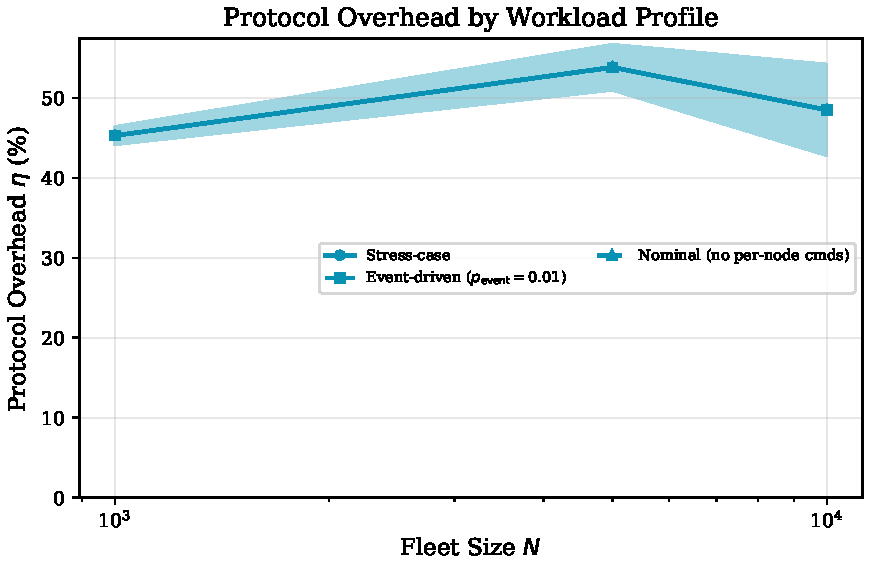
\includegraphics[width=\columnwidth]{fig-workload-comparison.pdf}
    \caption{Hierarchical overhead across three workload profiles. The $9\times$ stress-to-nominal spread bounds the design envelope.}
    \label{fig:workload}
\end{figure}

\textbf{Campaign duty factor.} The stress-case assumes continuous commands ($d = 1$, every cycle). In practice, maneuver campaigns (orbit-raising, collision avoidance) are episodic. A campaign duty factor $d \in [0,1]$ gates command generation per cycle (Bernoulli with probability $d$), yielding $\eta(d) = \eta_0 + d \cdot \eta_{\text{cmd}}$ (Eq.~\ref{eq:eta_canonical}). Table~\ref{tab:duty_factor} shows $\eta$ across the operational range. For routine operations ($d = 0.01$), overhead is negligibly above nominal; even intensive reconfiguration ($d = 0.10$) adds only ${\sim}4\%$. The stress-case ($d = 1$) remains useful as a strict upper bound.

\textbf{Representative campaign scenarios.} Three worked examples anchor $d$ in concrete mission phases: (1)~\emph{Orbit-raising} ($d = 0.05$, $L_{\text{on}} = 500$~cycles/83~min, $2 \times 7$~d/yr): annual average $\eta \approx 7\%$, peak $\eta = 7.1\%$. (2)~\emph{Station-keeping} ($d = 0.01$, $L_{\text{on}} = 50$~cycles/8~min, weekly): $\eta \approx 5.4\%$, peak $\eta = 5.4\%$. (3)~\emph{Collision avoidance} ($d \to 1.0$ during event, $L_{\text{on}} = 6$~cycles/1~min, ${\sim}12$ events/yr): background $\eta \approx 5\%$, peak $\eta = 46\%$ (stress bound). Routine operations thus occupy $\eta \approx 5$--$10\%$; the 46\% stress-case is episodic ($<$1\% of operational time).

\textbf{Empirical anchoring.} ESA's Space Debris Office reports ${\sim}300$ collision avoidance maneuvers per year across ${\sim}30$ ESA spacecraft~\cite{esa_space_env}, yielding a per-spacecraft maneuver cadence of ${\sim}10$/yr---consistent with our collision-avoidance $d$ scenario (${\sim}12$ events/yr). Starlink performs coordinated orbit-raising over 1--3~week windows after batch deployments, corresponding to $d \approx 0.02$--$0.10$ during the raising phase. These operational analogues place routine $d$ firmly in the $0.01$--$0.10$ range for LEO constellations.

\textbf{Temporal correlation.} The Bernoulli model assumes i.i.d.\ duty-factor draws; real campaigns exhibit temporal correlation. We implement an ON/OFF Markov alternative (geometric ON duration $L_{\text{on}}$ cycles, OFF duration $L_{\text{off}} = L_{\text{on}}(1-d)/d$) that preserves marginal $d$ but produces temporally correlated bursts. Fig.~\ref{fig:coordinator_buffer_cdf} confirms that ON/OFF ($L_{\text{on}} = 100$) produces heavier tails than Bernoulli at identical $d = 0.10$: the P99 coordinator ingress increases by ${\sim}15\%$, relevant for buffer sizing. The Bernoulli model is exact for mean $\eta$ and optimistic for peak buffer occupancy.

\begin{table}[t]
    \centering
    \caption{Overhead vs.\ Campaign Duty Factor ($k_c = 100$, $\gamma_{24} = 0.760$ reference)}
    \label{tab:duty_factor}
    \begin{tabular}{@{}lrrrrl@{}}
        \toprule
        $d$ & $\eta$ & $\eta_{\text{total}}$ & $\eta_{\text{total}}/\gamma$ & \textbf{TDMA?} & \textbf{Interpretation} \\
        \midrule
        0.00 & 5.0\% & 25.5\% & 33.6\% & No & Nominal \\
        0.01 & 5.4\% & 25.9\% & 34.1\% & No & Routine ops \\
        0.05 & 7.1\% & 27.6\% & 36.3\% & No & Orbit-raising \\
        0.10 & 9.1\% & 29.6\% & 38.9\% & No & Intensive reconfig \\
        0.50 & 25.5\% & 46.0\% & 60.5\% & Yes & Extended campaign \\
        1.00 & 46.0\% & 66.5\% & 87.5\% & Yes & Continuous (bound) \\
        \bottomrule
        \multicolumn{6}{@{}p{0.92\columnwidth}@{}}{\footnotesize $\eta(d) = \eta_0 + d \cdot \eta_{\text{cmd}}$; $\eta_{\text{cmd}} = 41\%$; baseline 20.5\%. TDMA required when $\eta_{\text{total}}/\gamma > 50\%$ (half-duplex margin).}
    \end{tabular}
\end{table}

\textbf{$\eta_0$ audit.} $\eta_0$ components: heartbeats 5.1\%~\cite{das_swim}, summaries 0.4\%, election $< 0.1\%$ (sum: 5.6\%); DES measures 5.0\%. The 0.5~pp gap: coordinators (1\% of fleet at $k_c = 100$) do not send status/heartbeat to themselves; fleet-average saving $= 0.01 \times (256 + 64) \times 8 / (1000 \times 10) = 0.026$~pp per component, $\approx 0.5$~pp total accounting for summary self-exclusion. Commands account for $>$60\% of stress-case traffic, summaries $<$1\%.

\textbf{Distributed planning.} 3-round Raft consensus~\cite{ongaro_raft} adds $\eta_{\text{consensus}} \approx 30.7\%$, competing with centralized $\eta_{\text{cmd}} = 41\%$; the ``topology-invariant'' conclusion holds only under centralized broadcast semantics.

\subsection{DES Distributional Analysis}
\label{sec:overhead_verification}

\subsubsection{Scaling Behavior and Implementation Consistency}

DES matches closed-form to $<$0.1\% at all fleet sizes $10^3$--$10^5$ (Table~\ref{tab:inflection}). This agreement is expected by construction: both compute the same sizing equations. The DES's independent contribution is \emph{distributional}: Fig.~\ref{fig:coordinator_buffer_cdf} shows that under stochastic duty-factor campaigns ($d = 0.10$) with GE burst losses, coordinator ingress variability is bimodal---most cycles near baseline, active cycles at full load---a property not captured by the closed-form mean. The ON/OFF campaign variant produces heavier tails (${\sim}15\%$ higher P99) relevant for buffer sizing.

\begin{figure}[t]
    \centering
    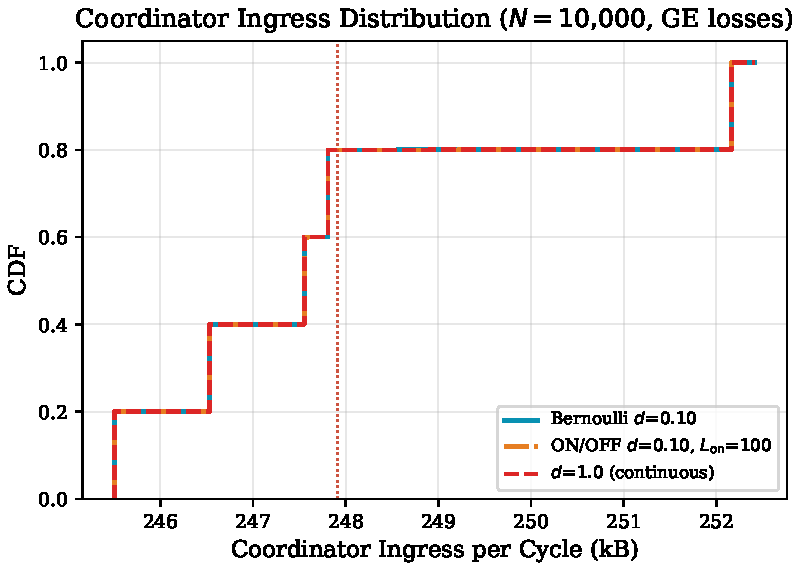
\includegraphics[width=\columnwidth]{fig-coordinator-buffer-cdf.pdf}
    \caption{CDF of per-cycle coordinator ingress bytes ($N = 10{,}000$, $k_c = 100$, GE losses). Bernoulli $d = 0.10$ (solid): bimodal, ${\sim}90\%$ of cycles at baseline. ON/OFF $d = 0.10$, $L_{\text{on}} = 100$ (dash-dot): heavier tail from sustained bursts. Continuous $d = 1.0$ (dashed): all cycles at full load. Vertical lines: closed-form means.}
    \label{fig:coordinator_buffer_cdf}
\end{figure}

\begin{table}[t]
    \centering
    \caption{Hierarchical Communication Overhead Scaling ($k_c = 100$)\textsuperscript{a}}
    \label{tab:inflection}
    \begin{tabular}{@{}lcccc@{}}
        \toprule
        \textbf{Fleet Size} & \textbf{$\eta_{\text{DES}}$ (\%)} & \textbf{$\eta_{\text{analytic}}$ (\%)} & \textbf{$\Delta$ (\%)} & \textbf{$\eta_{\text{eff}}$ (\%)}\textsuperscript{b} \\
        \midrule
        $10^3$--$10^5$\textsuperscript{c} & 46.0 & 46.1 & $<$0.1 & 51--66 \\
        \midrule
        \multicolumn{5}{@{}l}{\emph{With exception-based telemetry ($p_{\text{exc}} = 0.30$)}} \\
        $10^4$--$10^5$ & 14.0 & 13.8 & $<$1.5 & 16--20 \\
        \bottomrule
        \multicolumn{5}{@{}p{0.92\columnwidth}@{}}{\footnotesize\textsuperscript{a}30 MC replications, SD~$< 0.001\%$. \textsuperscript{b}$\eta_{\text{eff}} = \eta_{\text{DES}} / \gamma$ for $\gamma \in [0.7, 0.9]$. \textsuperscript{c}$\eta = 46.0\%$ at all 10 fleet sizes ($10^3$ through $10^5$); scale-invariant by construction.}
    \end{tabular}
\end{table}

\subsubsection{Analytical Cross-Check}
\label{sec:validation_crosscheck}

Exception telemetry reduces overhead linearly: $\eta(p_{\text{exc}}) \approx p_{\text{exc}} \times \eta(1.0)$ (verified at 6 configurations; all errors $\leq 1\%$; Fig.~\ref{fig:scaling_trajectory}).

\begin{figure}[t]
    \centering
    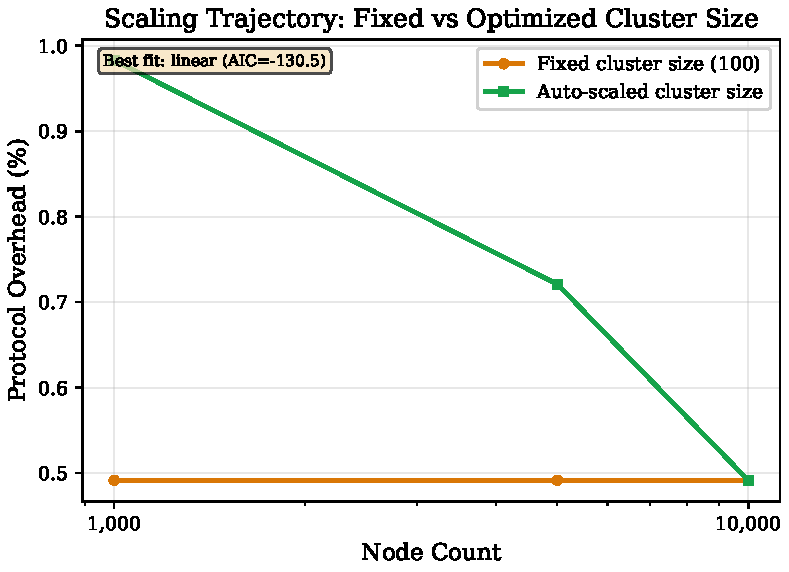
\includegraphics[width=\columnwidth]{fig-scaling-trajectory.pdf}
    \caption{Overhead trajectory (log-linear, DES-measured). Hierarchical $\eta \approx 46\%$ constant across $10^3$--$10^5$. Dashed: exception telemetry.}
    \label{fig:scaling_trajectory}
\end{figure}

\subsubsection{Parametric Sensitivity}
\label{sec:sensitivity}

Fig.~\ref{fig:sensitivity} presents parametric sensitivity: overhead scales linearly with $r$; at $\gamma = 0.7$, hierarchical reaches ${\sim}66\%$; at $\gamma < 0.5$ (CSMA), stress-case exceeds capacity.

\begin{figure}[t]
    \centering
    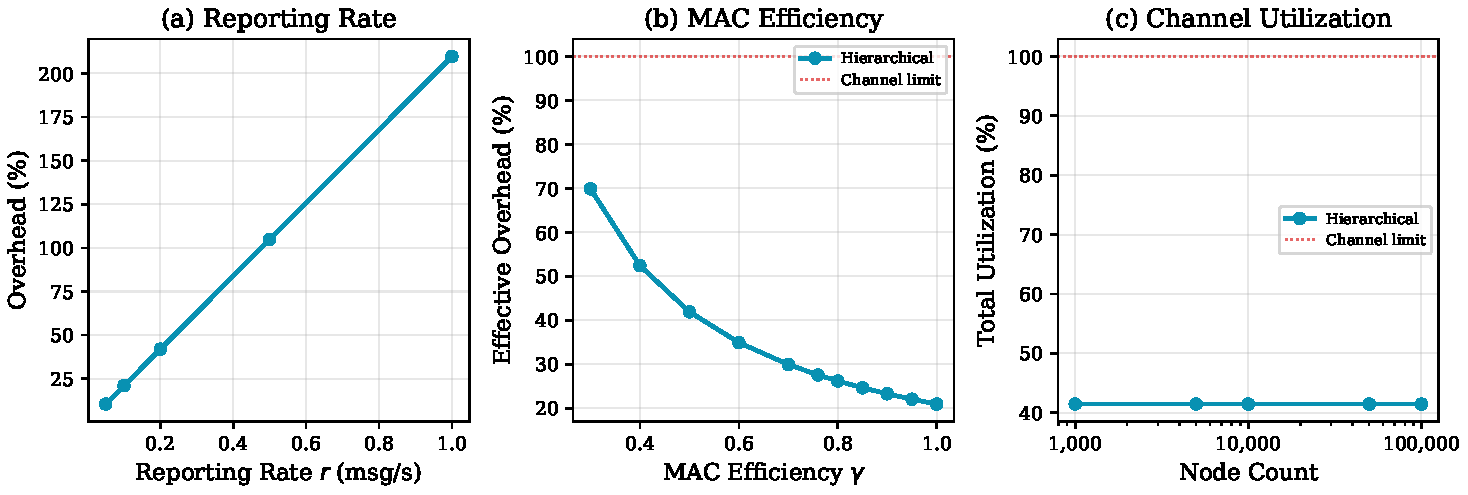
\includegraphics[width=\columnwidth]{fig-sensitivity-sweep.pdf}
    \caption{Parametric sensitivity. (a) Overhead vs.\ reporting rate. (b) MAC efficiency $\gamma$ vs.\ effective overhead. (c) Total channel utilization.}
    \label{fig:sensitivity}
\end{figure}

\subsection{Topology Comparison and Baselines}
\label{sec:topology_comparison}

Table~\ref{tab:topology_comparison} and Fig.~\ref{fig:overhead_scaling} summarize scaling behavior.

\textbf{Centralized baseline ($c = N/k_c$).} Centralized processing does not diverge until $N \approx 10^6$ under $M/D/c$. This model captures compute-queue scalability only---not uplink scheduling or ground contact availability \cite{wertz_smad}.

\textbf{Latency.} Within-cycle queueing: ${\sim}260$~ms mean ($D[k_c]/D/1$ batch: propagation 1.7~ms $+$ processing 5~ms/msg $+$ batch wait $k_c s_{\text{proc}}/2$), P95~$\approx 500$~ms. AoI: 44--441~s (Table~\ref{tab:aoi_results}). Centralized round-trip is lower; the hierarchical advantage is fault tolerance.

\begin{table}[t]
    \centering
    \caption{Coordination Topology Comparison}
    \label{tab:topology_comparison}
    \begin{tabular}{@{}lp{2.2cm}cc@{}}
        \toprule
        \textbf{Architecture} & \textbf{Scalability Limit} & \textbf{$O_{\text{protocol}}$\textsuperscript{a}} & \textbf{Failure Mode} \\
        \midrule
        \multicolumn{4}{@{}l}{\emph{Reference Bounds}} \\
        \;\;Centralized ($c\!=\!1$, bound)  & ${\sim}10{,}000$\textsuperscript{b}  & ---\textsuperscript{d}  & Single point \\
        \;\;Centralized ($c\!=\!N/k_c$)     & ${\sim}10^6$\textsuperscript{c}  & ---\textsuperscript{d}  & Single point \\
        \;\;Global-State Mesh (UB) & ${\sim}1{,}000$ & $>$100\% & Distributed (99.99\%) \\
        \midrule
        \multicolumn{4}{@{}l}{\emph{Architecture Under Study}} \\
        \;\;Hierarchical & $10^5$ (validated)    & 5--46\%   & Graceful (99.5\%) \\
        \bottomrule
        \multicolumn{4}{@{}p{0.85\columnwidth}@{}}{\footnotesize\textsuperscript{a}Protocol overhead beyond the topology-invariant 20.5\% baseline. Hierarchical range: ${\sim}5\%$ (exception telemetry, $p_{\text{exc}} = 0.10$) to ${\sim}46\%$ (stress-case full reporting).} \\
        \multicolumn{4}{@{}p{0.85\columnwidth}@{}}{\footnotesize\textsuperscript{b}Processing limit at $c\!=\!1$; propagation/spectrum limits persist. \textsuperscript{c}Realistic provisioning ($c = N/k_c$, $\rho \leq 0.7$); binding constraint is uplink spectrum and latency, not processing. \textsuperscript{d}Not applicable (compute-queue model only). A sectorized mesh ($\eta = 65$--$67\%$, local-neighbor monitoring only, Section~\ref{sec:sectorized_mesh_model}) is plotted in Fig.~\ref{fig:overhead_scaling} for reference but is not functionally comparable.}
    \end{tabular}
\end{table}

\begin{figure}[t]
    \centering
    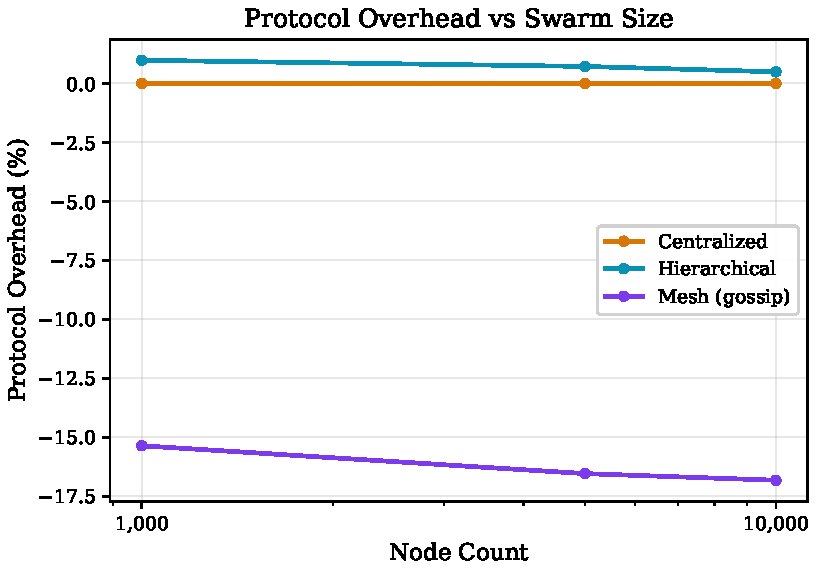
\includegraphics[width=\columnwidth]{fig-overhead-vs-nodes.pdf}
    \caption{Overhead vs.\ node count (log--log). Centralized ($c\!=\!1$) is \emph{compute-queue only}---divergence reflects processing, not communications. Mesh saturates; hierarchical stays at ${\sim}46\%$.}
    \label{fig:overhead_scaling}
\end{figure}


\textbf{Bandwidth--robustness tradeoff.} The hierarchy saves bandwidth via $1/k_c$ aggregation but depends on coordinator availability (99.5\%); the mesh provides local robustness at higher overhead with narrower scope (Table~\ref{tab:capability_matrix}). The hierarchy achieves $\gamma_{24} = 0.760$ via coordinator-assigned TDMA; decentralized architectures would require distributed TDMA coordination or CSMA/CA ($\gamma \approx 0.3$--$0.5$).

\begin{table}[t]
    \centering
    \caption{Functional Capability Matrix}
    \label{tab:capability_matrix}
    \begin{tabular}{@{}lcccc@{}}
        \toprule
        \textbf{Function} & \textbf{Cent.} & \textbf{Hier.} & \textbf{Mesh} & \textbf{Global} \\
        \midrule
        Fleet command dissem. & \checkmark & \checkmark & --- & --- \\
        Full cluster awareness & \checkmark\textsuperscript{a} & \checkmark & --- & \checkmark \\
        Local neighbor monitor & --- & \checkmark & \checkmark & \checkmark \\
        Summary aggregation & \checkmark\textsuperscript{a} & \checkmark & --- & --- \\
        No coordinator depend. & --- & --- & \checkmark & \checkmark \\
        Fits 1~kbps budget & ---\textsuperscript{b} & \checkmark & \checkmark & --- \\
        \bottomrule
        \multicolumn{5}{@{}p{0.85\columnwidth}@{}}{\footnotesize\textsuperscript{a}At ground; not in-orbit autonomous. \textsuperscript{b}Uplink-limited, not budget-limited.}
    \end{tabular}
\end{table}

\textbf{Comparability caveat.} The four architectures serve as analytical bounds, not competing designs. The centralized baseline models compute-queue scalability only, omitting the binding constraints of uplink spectrum and ground-contact windows; it should not be interpreted as ``centralized is feasible to $10^6$.'' The global-state mesh models worst-case full-state convergence---an intentional upper bound on decentralized overhead. The sectorized mesh provides local-neighbor monitoring only (no cluster-wide command or aggregation; Table~\ref{tab:capability_matrix}). Quantitative comparisons in Fig.~\ref{fig:overhead_scaling} and Table~\ref{tab:topology_comparison} are across these functionally distinct scopes; practitioners should select the baseline matching their operational requirements.

\subsection{Cluster, Duty Cycle, and Link Sensitivity}

\subsubsection{Cluster Size}

Protocol overhead is nearly invariant to $k_c$: $\eta = 46.0\%$ at $k_c \in \{50, 100, 200, 500\}$ ($\pm 0.1\%$, 30 MC replications). The trade-off is \emph{latency}: $k_c = 50$ increases regional queueing to 675~ms (vs.\ 508~ms at $k_c = 100$). $k_c = 100$--$200$ is favorable (Fig.~\ref{fig:cluster_opt}).

\begin{figure}[t]
    \centering
    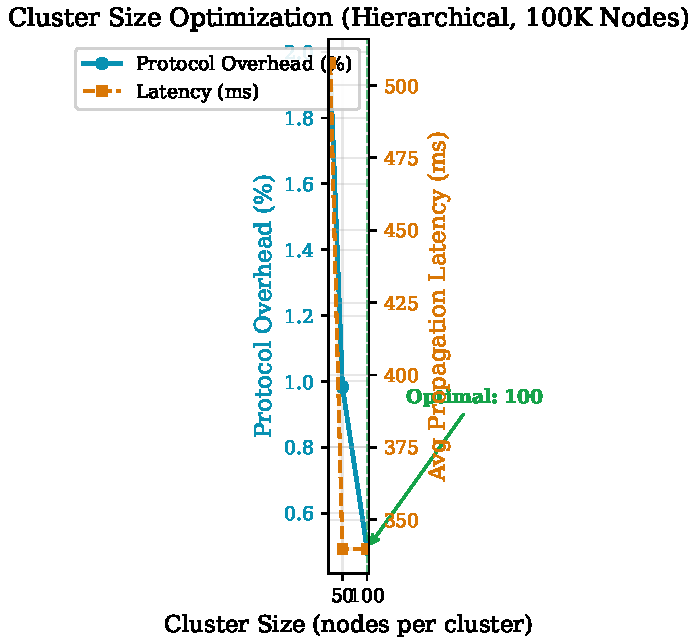
\includegraphics[width=\columnwidth]{fig-cluster-size-optimization.pdf}
    \caption{Cluster size sensitivity: $\eta$ invariant ($\pm 0.1\%$); latency drives the trade-off. $k_c = 100$--$200$ favorable.}
    \label{fig:cluster_opt}
\end{figure}

\subsubsection{Coordinator Duty Cycle}

The 24--48~h duty cycles occupy the Pareto frontier (Fig.~\ref{fig:duty_pareto}): power CV 12--18\%, handoff success $\geq 99.5\%$, system availability $\geq 99.2\%$ (two-state Markov, MTTF $= 50$~yr~\cite{castet_smallsat_reliability}). Shorter cycles (1--6~h) increase handoff cost without improving availability; longer (7~d) degrades power uniformity to 35\% CV. The 99.5\% in Table~\ref{tab:topology_comparison} conservatively accounts for cascading effects.

\begin{figure}[t]
    \centering
    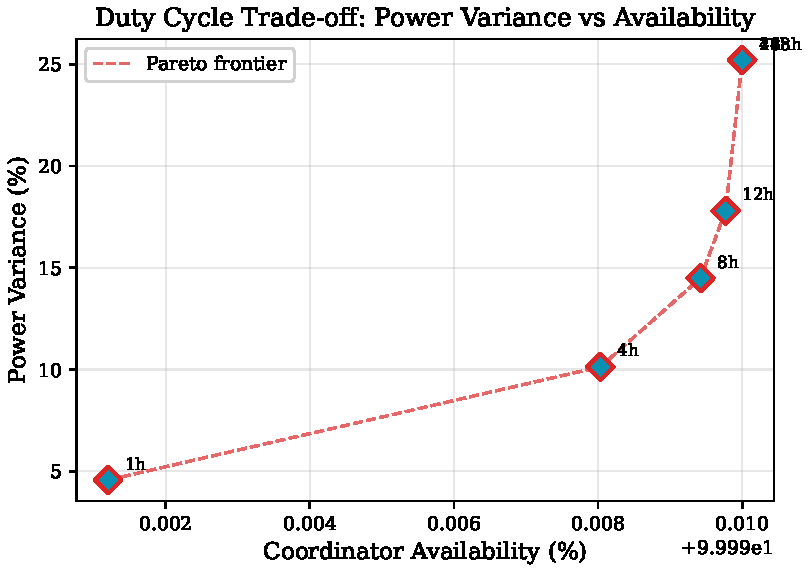
\includegraphics[width=\columnwidth]{fig-duty-cycle-pareto.pdf}
    \caption{Duty cycle trade-off in the power variance--system availability space. The 24\,h and 48\,h configurations offer the best balance.}
    \label{fig:duty_pareto}
\end{figure}

\subsubsection{Link Availability}

Table~\ref{tab:link_availability} summarizes coordination success under Bernoulli losses. Retransmission ($M_r = 2$) results are byte-budget delivery rates; TDMA airtime is not enforced. \textbf{Regime~A} ($\geq$10~kbps or $k_c \leq 30$): retransmissions fit in the superframe. \textbf{Regime~B} (RF-backup, 24--30~kbps, $k_c = 100$): effective $M_r = 0$ intra-cycle; recovery is inter-cycle (Section~\ref{sec:ge_link}).

\begin{table}[t]
    \centering
    \caption{Coordination Success vs.\ Link Availability ($N = 10^4$, $k_c = 100$). $M_r = 2$ columns apply to \textbf{Regime~A only} ($\geq$10~kbps or $k_c \leq 30$); for RF-backup Regime~B (24~kbps, $k_c = 100$), use $M_r = 0$ columns.}
    \label{tab:link_availability}
    \begin{tabular}{@{}lccccc@{}}
        \toprule
        \textbf{$p_{\text{link}}$} & \multicolumn{2}{c}{\textbf{Msg.\ Delivery (\%)}\textsuperscript{b}} & \multicolumn{2}{c}{\textbf{Delivered $\eta$ (\%)}} & \textbf{Offered}\textsuperscript{a} \\
        \cmidrule(lr){2-3} \cmidrule(lr){4-5}
         & $M_r\!=\!0$ & $M_r\!=\!2$ & $M_r\!=\!0$ & $M_r\!=\!2$ & $M_r\!=\!2$ \\
        \midrule
        1.0  & 100.0 & 100.0 & 46.0 & 46.0 & 46.0 \\
        0.9  & 89.9  & 99.9  & 41.3 & 46.0 & 51.1 \\
        0.8  & 79.9  & 99.3  & 36.8 & 45.7 & 57.0 \\
        0.7  & 69.8  & 98.0  & 32.1 & 45.1 & 63.9 \\
        0.6  & 59.7  & 95.8  & 27.5 & 44.1 & 71.8 \\
        0.5  & 49.9  & 92.9  & 23.0 & 42.7 & 80.5\textsuperscript{b} \\
        0.4  & 39.9  & 89.0  & 18.4 & 40.9 & 90.2\textsuperscript{b} \\
        \bottomrule
        \multicolumn{6}{@{}p{0.95\columnwidth}@{}}{\footnotesize \textsuperscript{a}Including retransmissions. \textsuperscript{b}Per-message rate; per-cycle $\approx (1 - p_{\text{loss}})^{k_c}$.}
    \end{tabular}
\end{table}

\label{sec:link_availability}



%% ===========================================================================
%% SECTION 4-J: STANDARDS-GROUNDED GAMMA DERIVATION
%% ===========================================================================
\subsection{Standards-Grounded $\gamma$ Derivation}
\label{sec:packet_validation}

The message-layer models (analytical, DES, slot-sim) all implement the same sizing equations; their agreement is expected by construction. To anchor the MAC efficiency parameter in physical-layer standards rather than assuming it, we construct a packet-level TDMA simulator that derives $\gamma$ from CCSDS-standard framing.

\subsubsection{$\gamma$ Decomposition from Physical-Layer First Principles}

Each TDMA slot is decomposed into four sub-efficiencies (Table~\ref{tab:gamma_decomposition}):
\begin{equation}
    \gamma_{\text{total}} = \gamma_{\text{framing}} \times \gamma_{\text{FEC}} \times \gamma_{\text{guard}} \times \gamma_{\text{acq}}
    \label{eq:gamma_decomposition}
\end{equation}

\begin{table}[t]
    \centering
    \caption{$\gamma$ Decomposition from CCSDS Proximity-1 Framing ($S_{\text{eph}} = 256$~B, 24~kbps PHY)}
    \label{tab:gamma_decomposition}
    \footnotesize
    \begin{tabular}{@{}llcc@{}}
        \toprule
        \textbf{Component} & \textbf{Mechanism} & \textbf{Efficiency} & \textbf{Source} \\
        \midrule
        Framing & ASM+addr+ctrl+FCS: 104~b OH & 0.952 & CCSDS 211.0-B-5~\cite{ccsds_prox1} \\
        FEC & LDPC rate 7/8: 2152$\to$2460~b & 0.875 & CCSDS 131.0-B-4~\cite{ccsds_sync_coding} \\
        Guard & prop+turn+jitter: 4.7~ms & 0.956 & Prox-1 + geometry \\
        Acquisition & pointing dwell: 5~ms & 0.955 & Typical S-band ISL \\
        \midrule
        \textbf{Total derived} & & \textbf{0.760} & Product \\
        Slot-level (Eq.~\ref{eq:gamma_derived}) & & 0.949 & No FEC/acq \\
        \bottomrule
    \end{tabular}
\end{table}

The derived $\gamma = 0.760$ is below the $\gamma = 0.949$ from the slot-level model (Eq.~\ref{eq:gamma_derived}), confirming that FEC and antenna acquisition collectively consume ${\sim}20\%$ of slot capacity.

\textbf{Rate dependence.} $\gamma$ is weakly rate-dependent through the guard/acquisition term in Eq.~\ref{eq:gamma_general}: at 24~kbps, $\gamma_{24} = 0.760$; at 30~kbps, $\gamma_{30} = 0.745$ (guard and acquisition consume a larger \emph{bit-equivalent} fraction at higher PHY rates). We write $\gamma_{24}$ and $\gamma_{30}$ where the distinction matters; unsubscripted $\gamma$ denotes the general function $\gamma(R_{\text{PHY}})$ from Eq.~\ref{eq:gamma_general}. The 30~kbps feasibility conclusion is robust to this variation: required ingress at $\gamma_{30} = 0.745$ is 27.5~kbps $< 30$~kbps. Practitioners should evaluate Eq.~\ref{eq:gamma_general} at their specific PHY rate.

\subsubsection{Cross-Model Consistency}

At 30~kbps with $\gamma = 0.745$, all four models (analytical, DES, slot-level, packet-level) agree on ingress $\approx 9{,}445$~ms with $\approx 355$~ms margin (Table~\ref{tab:rate_feasibility}). At 24~kbps, slot-level and packet-level models confirm infeasibility (ingress exceeds $T_c$). ARQ coupling at 24~kbps produces 52.7\% deadline misses (Table~\ref{tab:tdma_joint_interaction}).

\subsubsection{FEC Rate Sensitivity}

FEC rate has first-order impact: rate-1/2 LDPC makes 30~kbps infeasible; rate-7/8 confirms 30~kbps as minimum viable; rate-1.0 (no FEC) makes 24~kbps feasible at higher BER. Practitioners select FEC appropriate to their link; Eq.~\ref{eq:gamma_general} accepts the resulting $\gamma$.

\subsubsection{Interpretation}

The standards-grounded $\gamma$ derivation reveals that the feasibility boundary is tighter than a message-layer-only analysis would suggest. At 24~kbps with CCSDS-standard framing (rate-7/8 LDPC, 5~ms acquisition dwell), $\gamma = 0.76$ places the superframe in the infeasible region of Table~\ref{tab:gamma_sensitivity}. The 30~kbps design point is confirmed as a physical necessity, not merely a design margin.

%% ===========================================================================
%% SECTION 5: DISCUSSION
%% ===========================================================================
\section{Discussion}

\subsection{Validation Gap and Open Questions}
\label{sec:validation_gap}

Table~\ref{tab:claim_map} maps each key result to its verification tier. We distinguish three tiers of evidence:
\begin{enumerate}
    \item \textbf{Internal consistency} (Tier~1): DES vs.\ analytical equations---same model, different implementation. Agreement ($<$0.1\%) is expected by construction; the DES additionally provides distributional analysis (Fig.~\ref{fig:coordinator_buffer_cdf}).
    \item \textbf{Cross-model anchoring} (Tier~2): The slot-level TDMA simulator introduces superframe timing and half-duplex partitioning absent from the analytical equations, revealing ARQ$\times$TDMA coupling (Table~\ref{tab:tdma_joint_interaction}). The packet-level $\gamma$ derivation (Section~\ref{sec:packet_validation}) anchors MAC efficiency in CCSDS standards rather than assuming it.
    \item \textbf{External validation} (Tier~3): Full MAC contention, antenna scheduling, and multi-cluster shared-medium effects require NS-3 packet-level simulation---absent from this work and explicitly scoped as future work.
\end{enumerate}

\begin{table}[t]
    \centering
    \caption{Claim Map by Verification Tier}
    \label{tab:claim_map}
    \footnotesize
    \begin{tabular}{@{}lcccccc@{}}
        \toprule
         & \multicolumn{3}{c}{\textbf{Tier~1 (Internal)}} & \multicolumn{2}{c}{\textbf{Tier~2 (Cross-Model)}} & \textbf{Tier~3} \\
        \cmidrule(lr){2-4} \cmidrule(lr){5-6} \cmidrule(lr){7-7}
        \textbf{Result} & \textbf{Analyt.} & \textbf{DES} & \textbf{Distrib.} & \textbf{Slot-sim} & \textbf{Pkt-Level} & \textbf{Ext.} \\
        \midrule
        $\eta_0 \approx 5\%$ & \S\ref{sec:workload_profiles} & $<$0.1\% & --- & --- & --- & --- \\
        $\eta_S \approx 46\%$ & \S\ref{sec:workload_profiles} & $<$0.1\% & CDF & --- & --- & --- \\
        Coord.\ 24--30~kbps & Eq.~\ref{eq:tdma_capacity} & --- & CDF & Exact & 24 infeas. & --- \\
        Margin 623~ms & Tbl.~\ref{tab:superframe} & --- & --- & Exact & --- & --- \\
        $\gamma$ sensitivity & Tbl.~\ref{tab:gamma_sensitivity} & --- & --- & Conf. & $\gamma\!=\!0.76$ & --- \\
        ARQ infeas.\ (GE) & Markov & --- & --- & 52.7\% & Conf. & --- \\
        1~kbps design & --- & --- & --- & --- & Link budget & --- \\
        AoI P99 $= 440$~s & Eq.~\ref{eq:aoi_analytic} & Conf. & --- & --- & --- & --- \\
        GE P95 rec.\ 4 cyc. & Markov & Conf. & CDF & --- & --- & --- \\
        $L_{\text{cmd}}(q)$ stagger & Eq.~\ref{eq:unicast_stagger_q} & --- & --- & Conf. & --- & --- \\
        TDMA decoupling & --- & --- & --- & ($M_r\!=\!0$) & --- & --- \\
        ARQ coupling & --- & --- & --- & ($M_r\!\geq\!1$) & --- & --- \\
        $T_c^{\text{fleet}}$ reuse & Eq.~\ref{eq:fleet_reuse} & --- & --- & --- & --- & NS-3 \\
        Antenna sched. & --- & --- & --- & --- & --- & Future \\
        MAC contention & --- & --- & --- & --- & --- & Future \\
        \bottomrule
    \end{tabular}
\end{table}

\subsection{Limitations}
\label{sec:limitations}

\textbf{Physical-layer abstraction.} MAC contention, link acquisition, and Earth-occlusion outages are not modeled. \textbf{Priority queueing:} equal-priority messages; collision alerts should receive priority. \textbf{Failure models:} i.i.d.\ exponential; correlated modes are future work.

\textbf{Dynamic topology.} J2 perturbation analysis (Walker constellation: $53^\circ$, 550~km, 72~planes $\times$ 22~sats) shows co-orbital clusters experience zero re-association; cross-plane events occur at ${\sim}0.014$/orbit fleet-wide (${\sim}347$-day period per boundary). Re-association overhead: 14.8~kB (Raft election $+$ state handoff), amortized $<$0.3\% of byte budget; AoI transient 33~s ($<$8\% of P99). Cluster membership is fixed in the DES; dynamic membership is future work.


\subsection{Message-Layer Design Equations Summary}

For convenience, the key message-layer sizing relationships are collected here. All values assume message-layer operation; multiply bandwidth by $1/\gamma$ for MAC overhead ($\gamma_{24} = 0.760$, $\gamma_{30} = 0.745$; standards-derived, Section~\ref{sec:packet_validation}; Table~\ref{tab:rate_feasibility}). Practitioners may compute $\gamma$ for their specific link from:
\begin{equation}
    \gamma = \frac{S \times 8}{\dfrac{S \times 8 + O_{\text{frame}}}{R_{\text{FEC}}} + (T_{\text{guard}} + T_{\text{acq}}) \times R_{\text{PHY}} \times 10^{-3}}
    \label{eq:gamma_general}
\end{equation}
\noindent where $S$ is payload bytes, $O_{\text{frame}}$ is framing overhead (bits), $R_{\text{FEC}}$ is FEC code rate, $T_{\text{guard}}$/$T_{\text{acq}}$ are guard and acquisition times (ms), $R_{\text{PHY}}$ is PHY rate (bps), and the $10^{-3}$ converts ms$\cdot$bps to bits. Equivalently, in the time domain:
\begin{equation}
    \gamma = \frac{T_{\text{payload}}}{T_{\text{slot}}} = \frac{T_{\text{payload}}}{T_{\text{payload}} + T_{\text{FEC}} + T_{\text{framing}} + T_{\text{guard}} + T_{\text{acq}}}
    \label{eq:gamma_time}
\end{equation}
\noindent where $T_{\text{payload}} = S \times 8 / R_{\text{PHY}}$ is the information-bit transmission time. For the default instantiation ($S = 256$~B, $R_{\text{PHY}} = 24$~kbps, LDPC 7/8): $T_{\text{payload}} = 85.3$~ms, $T_{\text{FEC}} = 12.2$~ms, $T_{\text{framing}} = 4.3$~ms, $T_{\text{guard}} = 4.7$~ms, $T_{\text{acq}} = 5.0$~ms; $T_{\text{slot}} = 111.5$~ms, $\gamma = 85.3/111.5 = 0.765 \approx 0.76$ (cf.\ Table~\ref{tab:gamma_decomposition}). Table~\ref{tab:rate_feasibility} evaluates the feasibility boundary across PHY rates. For CCSDS Proximity-1: $O_{\text{frame}} = 104$~bits, yielding $\gamma = 0.760$ at 24~kbps and $\gamma = 0.745$ at 30~kbps. For CCSDS TC Space Data Link (CLTU encoding): $O_{\text{frame}} = 64$~bits, yielding $\gamma = 0.79$---a 4\% improvement shifting the minimum viable PHY rate to ${\sim}28$~kbps.

\begin{table}[t]
    \centering
    \caption{PHY Rate Feasibility ($k_c = 100$, CCSDS Prox-1 Framing)}
    \label{tab:rate_feasibility}
    \footnotesize
    \begin{tabular}{@{}lccccc@{}}
        \toprule
        $R_{\text{PHY}}$ & $\gamma(R_{\text{PHY}})$ & Slot & Ingress & Margin & Feasible? \\
        (kbps) & & (ms) & (ms) & (ms) & \\
        \midrule
        24 & 0.760 & 115.5 & 11{,}435 & $-$1{,}635 & N \\
        30 & 0.745 & 95.4 & 9{,}445 & 355 & Y \\
        50 & 0.725 & 60.8 & 6{,}019 & 3{,}781 & Y \\
        \bottomrule
        \multicolumn{6}{@{}p{0.85\columnwidth}@{}}{\footnotesize Ingress $= (k_c - 1) \times \text{Slot}$; Margin $= T_c - \text{Ingress} - 200$~ms (egress). $\gamma$ computed from Eq.~\ref{eq:gamma_general} with rate-dependent guard/acquisition.}
    \end{tabular}
\end{table}

\begin{itemize}
\item \textbf{Overhead:} $\eta = \eta_0 + d \cdot \eta_{\text{cmd}}$; $\eta_0 \approx 5\%$; $\eta_{\text{cmd}} = p_{\text{cmd}} S_{\text{cmd}} \times 8 / (C_{\text{node}} T_c)$; $d \in [0,1]$ is the campaign duty factor (Table~\ref{tab:duty_factor}).
\item \textbf{Coordinator ingress:} $C_{\text{coord}} \geq (k_c - 1) S_{\text{eph}} \times 8 / T_c$ ($\geq 20.3$~kbps at defaults).
\item \textbf{AoI P99:} $T_c \lceil \ln(0.01) / \ln(1 - p_{\text{exc}}) \rceil$ (440~s at $p_{\text{exc}} = 0.10$).
\item \textbf{GE bad-state recovery:} $p_{\text{success}} = 1 - p_B^{M_r+1}$ (27.1\%); inter-cycle P95 $= 4$ cycles at $p_{BG} = 0.50$ (Fig.~\ref{fig:cross_cycle_recovery}).
\item \textbf{Safe-mode:} $\gamma_{\min} = \eta_{\text{total}}$; nominal survives Slotted ALOHA ($\gamma \approx 0.36$); stress requires $\gamma \geq 0.67$.
\item \textbf{Fleet reuse:} $T_c^{\text{fleet}} = \max(T_c, \lceil f_{\text{RF}} N / (k_c F R) \rceil T_c)$; non-binding at $f_{\text{RF}} \leq 1.2\%$.
\end{itemize}

\textbf{Coordination Feasibility Test.} Algorithm~\ref{alg:feasibility} provides a step-by-step decision procedure that synthesizes the two-layer framework into an actionable sizing workflow.

\begin{algorithm}[t]
\caption{Coordination Feasibility Test}
\label{alg:feasibility}
\begin{algorithmic}[1]
\REQUIRE $k_c$, $S_{\text{eph}}$, $T_c$, $p_{\text{cmd}}$, $S_{\text{cmd}}$, $d$, $R_{\text{PHY}}$, FEC/framing parameters
\ENSURE Minimum $R_{\text{PHY}}$, feasibility status, stagger cycles $L_{\text{cmd}}$
\STATE \textbf{Layer 1 -- Byte budget:}
\STATE $\eta_0 \leftarrow$ architecture overhead (heartbeats + summaries + election)
\STATE $\eta_{\text{cmd}} \leftarrow d \cdot p_{\text{cmd}} \cdot S_{\text{cmd}} \times 8\;/\;(C_{\text{node}} \cdot T_c)$
\STATE $\eta_{\text{total}} \leftarrow \eta_0 + \eta_{\text{cmd}} + 0.205$ \COMMENT{baseline telemetry}
\STATE \textbf{MAC translation:}
\STATE $\gamma \leftarrow \gamma(R_{\text{PHY}})$ via Eq.~(\ref{eq:gamma_general})
\IF{$\eta_{\text{total}} / \gamma < 0.50$}
    \STATE CSMA may suffice; TDMA optional
\ELSE
    \STATE TDMA required
\ENDIF
\STATE \textbf{Layer 2 -- TDMA airtime:}
\STATE $T_{\text{slot}} \leftarrow (S_{\text{eph}} \times 8 + O_{\text{frame}}) / (R_{\text{FEC}} \cdot R_{\text{PHY}}) + T_{\text{guard}} + T_{\text{acq}}$
\STATE $T_{\text{ingress}} \leftarrow (k_c - 1) \times T_{\text{slot}}$
\STATE $T_{\text{egress}} \leftarrow T_{\text{cmd}} + T_{\text{hb}} + T_{\text{sync}}$
\IF{$T_{\text{ingress}} + T_{\text{egress}} \leq T_c$}
    \STATE Feasible at $R_{\text{PHY}}$; margin $= T_c - T_{\text{ingress}} - T_{\text{egress}}$
\ELSE
    \STATE Increase $R_{\text{PHY}}$ and repeat from Step~6
\ENDIF
\STATE \textbf{Stagger assessment:}
\STATE $L_{\text{cmd}} \leftarrow \lceil k_c \cdot T_{\text{cmd}} / (T_c \cdot (1 - \alpha_{\text{RX}})) \rceil$ \COMMENT{unicast cycles}
\RETURN $R_{\text{PHY,min}}$, margin, $L_{\text{cmd}}$
\end{algorithmic}
\end{algorithm}

\textbf{Uncertainty at MAC boundary.} Physical-layer overheads enter through $1/\gamma$ ($= 1.32$). Second-order interactions (contention $\times$ loss, antenna scheduling $\times$ half-duplex) require NS-3 simulation.

%% ===========================================================================
%% SECTION 6: CONCLUSION
%% ===========================================================================
\section{Conclusion}

This study provides a message-layer sizing framework for hierarchical coordination in autonomous space swarms ($10^3$--$10^5$ nodes), decomposing feasibility into two layers: byte budget ($\eta$) and physical-layer schedulability ($\gamma$, TDMA airtime). The framework separates topology-dependent overhead ($\eta_0$) from workload-dependent command traffic ($\eta_{\text{cmd}}$) and characterizes correlated loss recovery via a Gilbert-Elliott Markov chain parameterized as a sensitivity study across $(p_{BG}, p_B)$.

Under the representative instantiation (Table~\ref{tab:sim_params}): $\eta_0 \approx 5\%$; routine operations ($d = 0.01$--$0.10$) yield $\eta \approx 5$--$10\%$; the continuous-duty bound ($d = 1$) gives $\eta_S \approx 46\%$ but applies $<$1\% of operational time; coordinator ingress ${\approx}27$~kbps at standards-derived $\gamma_{24} = 0.760$; GE inter-cycle P95 recovery in 4~cycles; AoI P99~$= 440$~s (95\% CI: $[438, 444]$~s). Standards-grounded $\gamma$ derivation (Section~\ref{sec:packet_validation}) anchors $\gamma_{24} = 0.760$ (and $\gamma_{30} = 0.745$) in CCSDS Proximity-1 framing (rate-7/8 LDPC), confirming 30~kbps as the minimum viable design point. Algorithm~\ref{alg:feasibility} synthesizes the sizing procedure into an actionable feasibility test. An ON/OFF Markov campaign model (Section~\ref{sec:workload_profiles}) extends the Bernoulli duty-factor to temporally correlated campaigns, showing heavier-tailed coordinator ingress. The framework's value lies in the complete sizing procedure---from message-layer byte budget through PHY schedulability to coordinator capacity (Algorithm~\ref{alg:feasibility})---rather than in any single overhead figure. The remaining NS-3 gap (MAC contention, antenna scheduling) is identified in Table~\ref{tab:claim_map}.

\section*{Data Availability}

Source code, configuration, MC datasets, TDMA slot-level simulator, packet-level TDMA simulator, and link budget calculator are at \url{https://github.com/projectdyson/dyson} (tag: \texttt{paper-02-v-cf}). Parameters: Table~\ref{tab:sim_params}. Environment: Python 3.12, NumPy~2.x, SciPy~1.x, Matplotlib~3.x. Total MC wall-clock time: ${\sim}90$~min on commodity hardware.

\section*{Acknowledgment}

An AI-assisted ideation exercise (Claude~4.6, Gemini~3~Pro, GPT-5.2; see \cite{dyson_multimodel}) motivated aspects of the coordinator architecture but is not validated here.

\begin{thebibliography}{00}

\bibitem{starlink_ops}
SpaceX, ``Application for modification of authorization for the SpaceX Gen2 NGSO satellite system,'' FCC Filing SAT-MOD-20230320-00028, Mar.\ 2023. See also: J.~McDowell, ``Jonathan's Space Report,'' planet4589.org (non-archival; accessed Feb.\ 2026).

\bibitem{esa_conjunction}
T.~Flohrer, H.~Krag, and S.~Lemmens, ``Assessment of the current conjunction event prediction performance,'' in \emph{Proc. 7th European Conf. Space Debris}, Darmstadt, Germany, 2017, pp.~1--8.

\bibitem{kuiper}
Amazon, ``Project Kuiper: An overview,'' 2023 (non-archival; accessed February 2026). [Online]. Available: \url{https://www.aboutamazon.com/what-we-do/devices-services/project-kuiper}

\bibitem{oneweb_mgmt}
C.~McLaughlin, ``OneWeb constellation management approach,'' in \emph{Proc. 35th Space Symposium}, Colorado Springs, CO, 2019.

\bibitem{oneil_1976}
G.~K.~O'Neill, \emph{The High Frontier: Human Colonies in Space}.\hskip 1em plus 0.5em minus 0.4em New York, NY, USA: Morrow, 1976.

\bibitem{badescu_2006}
V.~Badescu and R.~B.~Cathcart, Eds., \emph{Macro-Engineering: A Challenge for the Future}.\hskip 1em plus 0.5em minus 0.4em Springer, 2006.

\bibitem{lynch_distributed}
N.~A.~Lynch, \emph{Distributed Algorithms}.\hskip 1em plus 0.5em minus 0.4em San Francisco, CA, USA: Morgan Kaufmann, 1996.

\bibitem{brambilla_2013}
M.~Brambilla, E.~Ferrante, M.~Birattari, and M.~Dorigo, ``Swarm robotics: A review from the swarm engineering perspective,'' \emph{Swarm Intell.}, vol.~7, no.~1, pp.~1--41, Mar.~2013.

\bibitem{wertz_smad}
J.~R.~Wertz, D.~F.~Everett, and J.~J.~Puschell, Eds., \emph{Space Mission Engineering: The New SMAD}.\hskip 1em plus 0.5em minus 0.4em Hawthorne, CA, USA: Microcosm Press, 2011.

\bibitem{reynolds_1987}
C.~W.~Reynolds, ``Flocks, herds, and schools: A distributed behavioral model,'' in \emph{Proc. 14th Annu. Conf. Comput. Graph. Interact. Tech. (SIGGRAPH)}, 1987, pp.~25--34.

\bibitem{dorigo_2021}
M.~Dorigo, G.~Theraulaz, and V.~Trianni, ``Swarm robotics: Past, present, and future,'' \emph{Proc. IEEE}, vol.~109, no.~7, pp.~1152--1165, Jul.~2021.

\bibitem{dorigo_aco}
M.~Dorigo and T.~St\"{u}tzle, \emph{Ant Colony Optimization}.\hskip 1em plus 0.5em minus 0.4em Cambridge, MA, USA: MIT Press, 2004.

\bibitem{kennedy_pso}
J.~Kennedy and R.~Eberhart, ``Particle swarm optimization,'' in \emph{Proc. IEEE Int. Conf. Neural Netw.}, vol.~4, Perth, Australia, 1995, pp.~1942--1948.

\bibitem{karaboga_abc}
D.~Karaboga and B.~Basturk, ``A powerful and efficient algorithm for numerical function optimization: Artificial bee colony (ABC) algorithm,'' \emph{J. Global Optim.}, vol.~39, no.~3, pp.~459--471, 2007.

\bibitem{tolstaya_gnn}
E.~Tolstaya, F.~Gama, J.~Paulos, G.~Pappas, V.~Kumar, and A.~Ribeiro, ``Learning decentralized controllers for robot swarms with graph neural networks,'' in \emph{Proc. Conf. Robot Learn. (CoRL)}, 2020, pp.~671--682.

\bibitem{lasry_mfg}
J.-M.~Lasry and P.-L.~Lions, ``Mean field games,'' \emph{Japanese J. Math.}, vol.~2, no.~1, pp.~229--260, 2007.

\bibitem{huang_mfg}
M.~Huang, R.~P.~Malham\'{e}, and P.~E.~Caines, ``Large population stochastic dynamic games: Closed-loop McKean--Vlasov systems and the Nash certainty equivalence principle,'' \emph{Commun. Inf. Syst.}, vol.~6, no.~3, pp.~221--252, 2006.

\bibitem{li_decentralized}
Q.~Li, F.~Gama, A.~Ribeiro, and A.~Prorok, ``Graph neural networks for decentralized multi-robot path planning,'' in \emph{Proc. IEEE/RSJ Int. Conf. Intell. Robots Syst. (IROS)}, 2020, pp.~11785--11792.

\bibitem{darpa_offset}
DARPA, ``OFFensive Swarm-Enabled Tactics (OFFSET),'' 2022 (non-archival; accessed February 2026). [Online]. Available: \url{https://www.darpa.mil/program/offensive-swarm-enabled-tactics}

\bibitem{dod_replicator}
U.S. Dept.\ of Defense, ``Replicator initiative fact sheet,'' Aug.~2023 (non-archival; accessed February 2026). [Online]. Available: \url{https://www.defense.gov/News/Releases/}

\bibitem{iridium_arch}
K.~Maine, C.~Devieux, and P.~Swan, ``Overview of IRIDIUM satellite network,'' in \emph{Proc. WESCON}, 1995, pp.~483--490.

\bibitem{kleinrock_queueing}
L.~Kleinrock, \emph{Queueing Systems, Vol.~I: Theory}.\hskip 1em plus 0.5em minus 0.4em New York, NY, USA: Wiley, 1975.

\bibitem{demers_gossip}
A.~Demers, D.~Greene, C.~Hauser, W.~Irish, J.~Larson, S.~Shenker, H.~Sturgis, D.~Swinehart, and D.~Terry, ``Epidemic algorithms for replicated database maintenance,'' in \emph{Proc. 6th Annu. ACM Symp. Principles Distrib. Comput.}, 1987, pp.~1--12.

\bibitem{castet_smallsat_reliability}
J.-F.~Castet and J.~H.~Saleh, ``Satellite and satellite subsystems reliability: Statistical data analysis and modeling,'' \emph{Reliab. Eng. Syst. Safety}, vol.~94, no.~11, pp.~1718--1728, 2009.


\bibitem{dyson_multimodel}
Project Dyson Research Team, ``Multi-model AI deliberation for engineering design exploration: Methodology and case studies,'' 2025. [Online]. Available: \url{https://projectdyson.org/publications}

\bibitem{lamport_clocks}
L.~Lamport, ``Time, clocks, and the ordering of events in a distributed system,'' \emph{Commun. ACM}, vol.~21, no.~7, pp.~558--565, Jul.~1978.

\bibitem{ongaro_raft}
D.~Ongaro and J.~Ousterhout, ``In search of an understandable consensus algorithm,'' in \emph{Proc. USENIX Annu. Tech. Conf. (ATC)}, Philadelphia, PA, USA, 2014, pp.~305--319.

\bibitem{ccsds_prox1}
Consultative Committee for Space Data Systems, ``CCSDS 211.0-B-6: Proximity-1 space link protocol---data link layer,'' CCSDS, Blue Book, Sep.~2013.

\bibitem{handley_2018}
M.~Handley, ``Delay is not an option: Low latency routing in space,'' in \emph{Proc. 17th ACM Workshop Hot Topics Netw. (HotNets)}, Redmond, WA, USA, 2018, pp.~85--91.

\bibitem{darpa_blackjack}
DARPA, ``Blackjack program,'' 2023 (non-archival; accessed February 2026). [Online]. Available: \url{https://www.darpa.mil/program/blackjack}

\bibitem{das_swim}
A.~Das, I.~Gupta, and A.~Motivala, ``SWIM: Scalable weakly-consistent infection-style process group membership protocol,'' in \emph{Proc. Int. Conf. Dependable Syst. Netw. (DSN)}, Washington, DC, USA, 2002, pp.~303--312.

\bibitem{darpa_f6}
O.~Brown and P.~Eremenko, ``Fractionated space architectures: A vision for responsive space,'' in \emph{Proc. 4th Responsive Space Conf.}, Los Angeles, CA, USA, 2006, pp.~RS4-2006-1002.

\bibitem{golkar_federated}
A.~Golkar and I.~Lluch i~Cruz, ``The federated satellite systems paradigm: Concept and business case evaluation,'' \emph{Acta Astronautica}, vol.~111, pp.~230--248, Jun.--Jul.~2015.

\bibitem{olfati_consensus}
R.~Olfati-Saber and R.~M.~Murray, ``Consensus problems in networks of agents with switching topology and time-delays,'' \emph{IEEE Trans. Autom. Control}, vol.~49, no.~9, pp.~1520--1533, Sep.~2004.

\bibitem{ren_beard}
W.~Ren and R.~W.~Beard, ``Consensus seeking in multiagent systems under dynamically changing interaction topologies,'' \emph{IEEE Trans. Autom. Control}, vol.~50, no.~5, pp.~655--661, May~2005.

\bibitem{ccsds_bpv7}
Consultative Committee for Space Data Systems, ``CCSDS 734.2-B-1: Bundle protocol version 7,'' CCSDS, Blue Book, Sep.~2020.

\bibitem{akyildiz_isl}
I.~F.~Akyildiz, E.~Ekici, and G.~Yue, ``A distributed multicast routing scheme for multi-layered satellite IP networks,'' \emph{Wireless Netw.}, vol.~9, no.~5, pp.~535--544, Sep.~2003.

\bibitem{del_portillo_mega}
I.~del~Portillo, B.~G.~Cameron, and E.~F.~Crawley, ``A technical comparison of three low Earth orbit satellite constellation systems to provide global broadband,'' \emph{Acta Astronautica}, vol.~159, pp.~123--135, Jun.~2019.

\bibitem{cerf_dtn}
V.~Cerf, S.~Burleigh, A.~Hooke, L.~Torgerson, R.~Durst, K.~Scott, K.~Fall, and H.~Weiss, ``Delay-tolerant networking architecture,'' IETF, RFC~4838, Apr.~2007.

\bibitem{esa_space_env}
ESA Space Debris Office, ``ESA's annual space environment report,'' ESA, GEN-DB-LOG-00288-OPS-SD, 2024.

\bibitem{kaul_aoi}
S.~Kaul, R.~Yates, and M.~Gruteser, ``Real-time status: How often should one update?'' in \emph{Proc. IEEE INFOCOM}, Orlando, FL, USA, 2012, pp.~2731--2735.

\bibitem{yates_aoi}
R.~D.~Yates, Y.~Sun, D.~R.~Brown, S.~K.~Kaul, E.~Modiano, and S.~Ulukus, ``Age of information: An introduction and survey,'' \emph{IEEE J. Sel. Areas Commun.}, vol.~39, no.~5, pp.~1183--1210, May~2021.

\bibitem{kadota_aoi}
I.~Kadota, A.~Sinha, E.~Uysal-Biyikoglu, R.~Singh, and E.~Modiano, ``Scheduling policies for minimizing age of information in broadcast wireless networks,'' \emph{IEEE/ACM Trans. Netw.}, vol.~26, no.~6, pp.~2637--2650, Dec.~2018.

\bibitem{vallado_astrodynamics}
D.~A.~Vallado, \emph{Fundamentals of Astrodynamics and Applications}, 4th~ed.\hskip 1em plus 0.5em minus 0.4em Hawthorne, CA, USA: Microcosm Press, 2013.

\bibitem{alfano_conjunction}
S.~Alfano, ``A numerical implementation of spherical object collision probability,'' \emph{J. Astronaut. Sci.}, vol.~53, no.~1, pp.~103--109, Jan.--Mar.~2005.

\bibitem{bhattacherjee_isl}
D.~Bhattacherjee, W.~Aqeel, I.~N.~Bozkurt, A.~Aguber, B.~Chandrasekaran, P.~B.~Godfrey, G.~Laughlin, B.~M.~Maggs, and A.~Singla, ``Gearing up for the 21st century space race,'' in \emph{Proc. 17th ACM Workshop Hot Topics Netw. (HotNets)}, Redmond, WA, USA, 2018, pp.~113--119.

\bibitem{ccsds_spp}
Consultative Committee for Space Data Systems, ``CCSDS 133.0-B-2: Space packet protocol,'' CCSDS, Blue Book, Jun.~2020.

\bibitem{nasa_dsa}
S.~Chien, J.~Doubleday, K.~L.~Wagstaff, D.~R.~Thompson, and S.~Schaffer, ``Distributed spacecraft autonomy,'' in \emph{Proc. IEEE Aerosp. Conf.}, Big Sky, MT, USA, 2024, pp.~1--10.

\bibitem{fraire_cgr}
J.~A.~Fraire, P.~G.~Madoery, and J.~M.~Finochietto, ``Contact graph routing in DTN space networks: Overview, enhancements and performance,'' \emph{IEEE Commun. Mag.}, vol.~59, no.~2, pp.~118--124, Feb.~2021.

\bibitem{heinzelman_leach}
W.~R.~Heinzelman, A.~Chandrakasan, and H.~Balakrishnan, ``Energy-efficient communication protocol for wireless microsensor networks,'' in \emph{Proc. 33rd Hawaii Int. Conf. Syst. Sci.}, Maui, HI, USA, 2000, pp.~1--10.

\bibitem{ieee_1012}
IEEE, ``IEEE Std 1012-2016: Standard for System, Software, and Hardware Verification and Validation,'' IEEE, New York, NY, USA, 2017.

\bibitem{lutz_1991}
E.~Lutz, D.~Cygan, M.~Dippold, F.~Dolainsky, and W.~Papke, ``The land mobile satellite communication channel---recording, statistics, and channel model,'' \emph{IEEE Trans. Veh. Technol.}, vol.~40, no.~2, pp.~375--386, May~1991.

\bibitem{itu_p681}
ITU-R, ``Recommendation ITU-R P.681-11: Propagation data required for the design of Earth-space land mobile telecommunication systems,'' Geneva, 2019.

\bibitem{leboudec_netcalc}
J.-Y.~Le~Boudec and P.~Thiran, \emph{Network Calculus: A Theory of Deterministic Queuing Systems for the Internet}.\hskip 1em plus 0.5em minus 0.4em Berlin, Germany: Springer, 2001.

\bibitem{ccsds_sfdp}
Consultative Committee for Space Data Systems, ``CCSDS 132.0-B-3: TM space data link protocol,'' CCSDS, Blue Book, Sep.~2020.

\bibitem{ccsds_sync_coding}
Consultative Committee for Space Data Systems, ``CCSDS 131.0-B-4: TM synchronization and channel coding,'' CCSDS, Blue Book, Sep.~2020.

\end{thebibliography}

\end{document}
